\documentclass[11pt, letterpaper]{article}
%\usepackage[T1]{fontenc}
%\usepackage{geometry}
%\geometry{verbose,a4paper,tmargin=15mm,bmargin=30mm,lmargin=30mm,rmargin=20mm}

\setlength{\oddsidemargin}{-.15in}
\setlength{\evensidemargin}{-.15in}
\setlength{\textwidth}{7.0in}
\setlength{\topmargin}{-0.5in}
\setlength{\textheight}{9.2in}

% \setlength{\oddsidemargin}{-.4in}
% \setlength{\evensidemargin}{-.4in}
% \setlength{\textwidth}{7.3in}
% \setlength{\topmargin}{-0.5in}
% \setlength{\textheight}{9.4in}

\usepackage{setspace}
%\doublespacing
\onehalfspacing

%\usepackage{pslatex}
\usepackage[bookmarks=true,bookmarksnumbered=true]{hyperref}
\usepackage{amsmath}
\usepackage{booktabs}
\usepackage{euscript}
\usepackage[]{graphicx}
\usepackage{multirow}
\usepackage{epsfig}
\usepackage{subfig}
\usepackage{amsfonts}
\usepackage{verbatim}
\usepackage{amssymb}
\usepackage{amsbsy}
\usepackage{physics}
\usepackage{dsfont}
\usepackage{url}
\usepackage{epstopdf}
\usepackage{enumitem}
\usepackage{tabularx}
\usepackage[usenames,dvipsnames]{color}
\usepackage[compact]{titlesec}
\usepackage[square,numbers,sort]{natbib}
\setlength{\bibsep}{-1pt}

\usepackage{algpseudocode}
\usepackage{algorithm}
\usepackage{wrapfig}

\usepackage{float}
\floatstyle{plaintop}
\restylefloat{table}


%\usepackage[margin=1cm]{geometry}
\usepackage{pgfgantt}
\usepackage{graphicx}
\usepackage{xcolor}
%\usetikzlibrary{positioning}
\usepackage[toc,page]{appendix}


\usepackage[]{algorithm2e}
\usepackage[ruled,vlined]{algorithm2e}
\SetKwInput{KwInput}{Input}                % Set the Input
\SetKwInput{KwOutput}{Output}  
\usepackage{tikz}
\usetikzlibrary{mindmap,backgrounds,decorations,positioning,shapes,shadows,arrows,chains}
\usetikzlibrary[positioning]
\usetikzlibrary{patterns}
\usetikzlibrary{arrows,chains,positioning,scopes,shapes.geometric,shapes.misc,shadows}

\usepackage{fancyhdr}

\newcommand{\degree}{\ensuremath{^\circ\,}}
\newcommand{\unit}[1]{\ensuremath{\, \mathrm{#1}}}
\newcommand{\etal}{\textit{et al.}}


\newcommand{\bm}[1]{\mbox{\boldmath{${#1}$}}}
\newcommand{\pd}[2]{{\frac{\partial {#1}}{\partial {#2}}}}
\newcommand{\pdd}[2]{{\frac{\partial^2 {#1}}{\partial {#2}^2}}}
\newcommand{\od}[2]{{\frac{{\rm{d}} {#1}}{{\rm{d}} {#2}}}}
\newcommand{\odd}[2]{{\frac{{\rm{d}}^2 {#1}}{{\rm{d}} {#2}^2}}}



\usepackage{tikz}
\usetikzlibrary{mindmap,backgrounds,decorations,positioning,shapes,shadows,arrows,chains}
\usetikzlibrary[positioning]
\usetikzlibrary{patterns}
\usetikzlibrary{arrows,chains,positioning,scopes,shapes.geometric,shapes.misc,shadows}

\usepackage{fancyhdr}
\pagestyle{fancy}

\usepackage[subfigure]{tocloft}

\setlength\cftparskip{-3pt}
%\setlength\cftbeforechapskip{0pt}

% \rfoot{\thepage}


\begin{document}

\iffalse

\begin{titlepage}
\thispagestyle{empty}
\renewcommand\thepage{}
{\centering
\large
%{\Large\bf Surrogate Modeling for Variable-Fidelity Multidisciplinary Design Optimization of Aircraft Configurations}\\
\begin{center}
	{\large\bf Multiple Kernel Kriging Methods for Aerospace Applications}
	%
	%% \underline the presenter
	%% \footnote for corr. author & e-mail should be placed after the last author
	%
	\newline
	Kehinde Sikirulai Oyetunde [20548072],  Sathi Sarveswara [20647048] ####
\end{center}
%\vspace{0.3cm}
%15 January 2014\\
}
%\vspace{1.5cm}
%\vspace{0.2cm}
\begin{small}
{\centering
\textbf{Abstract}\\
}
\vspace{0.2cm}
\begin{spacing}{1.2}
  \noindent 
        Computational fluid dynamics is used in aerospace industries to simulate computational experiments. The computations involve with CFD usually requires several iterations and could take days to solve depending on the size of the model. The heavy computational power required makes it difficult to solve certain design optimization problems. Kriging (Gaussian processes) are introduced to build high performance surrogates for such experiments using limited data. This report focuses on the development and use of machine learning techniques (Kriging) for small datasets. In specific, we used various kernels within Kriging formulations. Also, three multiple kernel methods are developed and benchmarked with four single kernels. A 8D and 16D CFD data which has the drag coefficient as its quantity of interest (QoI) is used. The composite kernel learning multiple kernel method performs best with lesser model error and computational times.
\end{spacing}

\end{small}
\end{titlepage}

\fi
% \pagebreak


% \thispagestyle{empty}
% \renewcommand\thepage{}
{\centering
\large
%{\Large\bf Surrogate Modeling for Variable-Fidelity Multidisciplinary Design Optimization of Aircraft Configurations}\\
\begin{center}
	{\large\bf Multiple Kernel Kriging Methods for Aerospace Applications}
	%
	%% \underline the presenter
	%% \footnote for corr. author & e-mail should be placed after the last author
	%
	\newline
	Kehinde Sikirulai Oyetunde [20548072],  Sathi Sarveswara [20647048] ####
\end{center}
%\vspace{0.3cm}
%15 January 2014\\
}
%\vspace{1.5cm}
%\vspace{0.2cm}
\begin{small}
{\centering
\textbf{Abstract}\\
}
\vspace{0.2cm}
\begin{spacing}{1.2}
  \noindent 
        Computational fluid dynamics is used in aerospace industries to simulate computational experiments. The computations involve with CFD usually requires several iterations and could take days to solve depending on the size of the model. The heavy computational power required makes it difficult to solve certain design optimization problems. Kriging (Gaussian processes) are introduced to build high performance surrogates for such experiments using limited data. This report focuses on the development and use of machine learning techniques (Kriging) for small datasets. In specific, we used various kernels within Kriging formulations. Also, three multiple kernel methods are developed and benchmarked with four single kernels. A 8D and 16D CFD data which have the drag coefficient as its quantity of interest (QoI) is used. The composite kernel learning multiple kernel method performs best with lesser model error and computational times.
\end{spacing}

\end{small}

\section{Introduction} 
	\label{intro}
The work done in this project is motivated by the heavy computational resource required for CFD simulations in the aerospace industries. Also, in part motivated by the need for machine learning techniques for appications with small datasets having a little as 1000 points. We developed Kriging models which are a variant of Gaussian process regression (Gpr) but with no noise. Hence, Kriging models are best suited for deterministic data obtainable in CFD simulations. CFD simulations are considered deterministic because same set of input will give same output. Our Kriging methods models the output as a realization of a Gaussian distribution. We used the Gaussian, exponential, Mat\'ern 3/2, Mat\'ern 5/2 kernels in building our models. Three multiple kernels methods are developed using the four single kernels to improve the performance of the Kriging models as well as reduce the bias from the individual kernels. Lastly, we compared the performance of the seven models (single and multiple kernel methods) on the two available datasets.

\section{Methods}
Kriging is used for approximating computationally expensive blackbox functions. The relationship between the input, $\boldsymbol{x}$, and the output, $\boldsymbol{y}$ of a blackbox function in Kriging, can be expressed as:
\begin{equation}
\label{kriging_eqn}
Y(x) = \mu(x) + Z(x),
\end{equation}
where $\mu(x)$ is the deterministic function approximating the mean trend of the output and Z(x) is the stochastic process which deviates from this trend. Z(x) has a zero mean and the covariance
$\text{Cov}\left[Z\left(\mathbf{x}\right),Z\left(\mathbf{x}'\right)\right]
= \sigma^2\mathbf{R}\left(\mathbf{x}, \mathbf{x}'\right)$. $\sigma^2$
is the process variance and $\mathbf{R}\left(\cdot, \cdot\right)$ is the
correlation matrix. The correlation
between the $i$-th and $j$-th samples can then be expressed as:
\begin{equation}
R_{ij}\left(\boldsymbol{h , \theta}\right) = \prod_{k=1}^{N_d}{R\left(h_{ij}^{\left(k\right)},\theta^{\left(k\right)}\right)}.
\label{eq:corrProduct}
\end{equation}
The vector of correlation parameters is denoted as
$\boldsymbol{\theta} = \left\{\theta^{\left(k\right)}\right\}, \, k=1,
\ldots N_d$. The value $h_{ij}^{\left(k\right)}$ is the distance
between two points in the $k^{\text{th}}$ dimension,
$\left|x_i^{\left(k\right)} - x_j^{\left(k\right)}\right|$.
For a simple kriging model with a constant trend, the mean and the variance of the prediction at a point $\boldsymbol{x}$ is expressed as;

\begin{equation}
m(\boldsymbol{x}) =  \mu + \boldsymbol{r}(\boldsymbol{x})^T\boldsymbol{R}^{-1}(\boldsymbol{y}-\boldsymbol{1}\mu)
\end{equation}

\begin{equation}
s^2(\boldsymbol{x}) =  \hat{\sigma}^2\left(1-\boldsymbol{r}(\boldsymbol{x})^T\boldsymbol{R}^{-1}\boldsymbol{r}(\boldsymbol{x})\right)
\end{equation}

\subsection{Kernels}
Kernels are used to capture the non-linear relationship that exist betweem the input \mathbf{x} and output, y. In this report, four kernels: the Gaussian, Exponential, Mat\'ern 3/2 and Mat\'ern 5/2 kernels are used for performance comparison and also to develop the various models. 

\begin{itemize}
	\item Gaussian	
	\begin{equation}
	R(\boldsymbol{h,\theta}) = \exp-\frac{1}{2}\left(\boldsymbol{\frac{h}{\theta}}\right)^2
	\end{equation}
	
	\item Exponential	
	\begin{equation}
	R(\boldsymbol{h,\theta}) = \exp-\frac{1}{2}\left(\boldsymbol{\frac{h}{\boldsymbol{\theta}}}\right)
	\end{equation}
	
	\item Matern 3/2
	\begin{equation}
	R(\boldsymbol{h,\theta}) = \left(1 + \frac{\sqrt{3}|\boldsymbol{h}|}{\boldsymbol{\theta}}\right)exp\left(-\frac{\sqrt{3}|\boldsymbol{h}|}{\boldsymbol{\theta}}\right)
	\end{equation} 
	
	\item Matern 5/2
	\begin{equation}
	R(\boldsymbol{h,\theta}) = \left(1 + \frac{\sqrt{5}|\boldsymbol{h}|}{\boldsymbol{\theta}} + \frac{5\boldsymbol{h}^2}{3\boldsymbol{\theta}^2}\right)exp\left(-\frac{\sqrt{5}|\boldsymbol{h}|}{\boldsymbol{\boldsymbol{\theta}}}\right)
	\end{equation} 
\end{itemize}
where $h$ is a function of distance $|x-x'|$ and $\boldsymbol{\theta}$ is the length scale

\subsection{Multiple kernel methods}
This generally refers to methods which uses more than one kernel or several instance of a kernel (with different parameters). We developed three multiple kernel methods; ensemble method, composite kernel learning (CKL), multidimensional composite kernel learning (MCKL) methods. The ensemble method~\cite{Palar2018,Palar2019a} which can either be global or local uses weights to combine different models.  We developed the ensemble method which uses corrected-Akaike information criterion (AICc)~\cite{Martin2005a} for global weight computations. The correction introduced takes into account the factor of sample size and increase the penalty for model complexity with small data sets. The ensemble method help to reduce error  and  bias in  the  model. Another method which we developed is the Composite Kernel Learning (CKL) method~\cite{Palar2019}. It involves the construction of new kernels by combinations of existing kernels. The technique aims at improving the approximation quality of models by avoiding the misspecification of kernels.


\begin{itemize}

\item \textbf{Ensemble method}: The predictions of each models are globally combined using equation \ref{ens}
	\begin{equation}
	\label{ens}
		\hat{y}_{ens}(x) = \sum_{i=1}^{K}w_i(x)\hat{y}_i(x)
	\end{equation}
The weight is computed; 
	\begin{equation}
		w_i = \frac{exp(-0.5\Delta AIC_i)}{\sum_{j=1}^{K}exp(-0.5\Delta AIC_j)}
	\end{equation}
where,
	\begin{equation}
		AIC = -2\ln(L) + 2N_f
	\end{equation}

	\begin{equation}
		AIC_c = AIC + \frac{2N_f^2 + 2N_f}{n - N_f-1}
	\end{equation}
	
	\begin{equation}
		\Delta AIC_i = AIC_i - AIC_{min}
	\end{equation}
	\begin{equation}
		N_f = len(\theta) + 2
	\end{equation}
	
    \item \textbf{Composite Kernel Learning (CKL)}: The weighted sum formulation of combined kernels as follows:
\begin{equation}
R_{CKL}(h) = \sum_{i=1}^{K}w_i(x)R_i(h)
\end{equation}

where $\textbf{w} = {w_1,w_2,...,w_K}^T $ is the non-negative weight vector that should satisfies the equality constraint $\sum_{i=1}^K w_i = 1$.

\item \textbf{Multidimensional Composite Kernel Learning (MCKL)}\\
The kernels for the MCKL formulations are combined using equation \ref{mckl_eq}
\begin{equation}
\label{mckl_eq}
    R_{ij}(\boldsymbol{\theta},h) = \prod\limits_{d=1}^{n}\sum_{i=1}^{m}w_{nm}R\left(\theta^{(d)},h_{ij}^{(d)}\right)
\end{equation}
where, \\
\begin{align*}\vb{w} = 
\mqty(
w_{1,1} & w_{1,2} & \cdots & w_{1,m} \\
w_{2,1} & w_{2,2} & \cdots & w_{2,m} \\
\vdots  & \vdots  & \ddots & \vdots  \\
w_{n,1} & w_{n,2} & \cdots & w_{n,m} )
\end{align*}
\end{itemize}



\section{Data}
For benchmarking purposes, we used the drag coefficient data obtained from the computational fluid dynamics computations of the TUDelft HPC cluster. The data contains both 8- and 16- dimensional shape parameters (input) and corresponding drag coefficient (output). The 8D and 16D data have 500 and 1000 points respectively. The scatter plot showing the distribution of the data is shown in Figure \ref{scatter} with the bottom row representing the cross-plot of the drag coefficient and the input variables.

\begin{figure}[!h]
	\begin{center}
		\vspace{-10pt}
		\mbox{ \subfloat{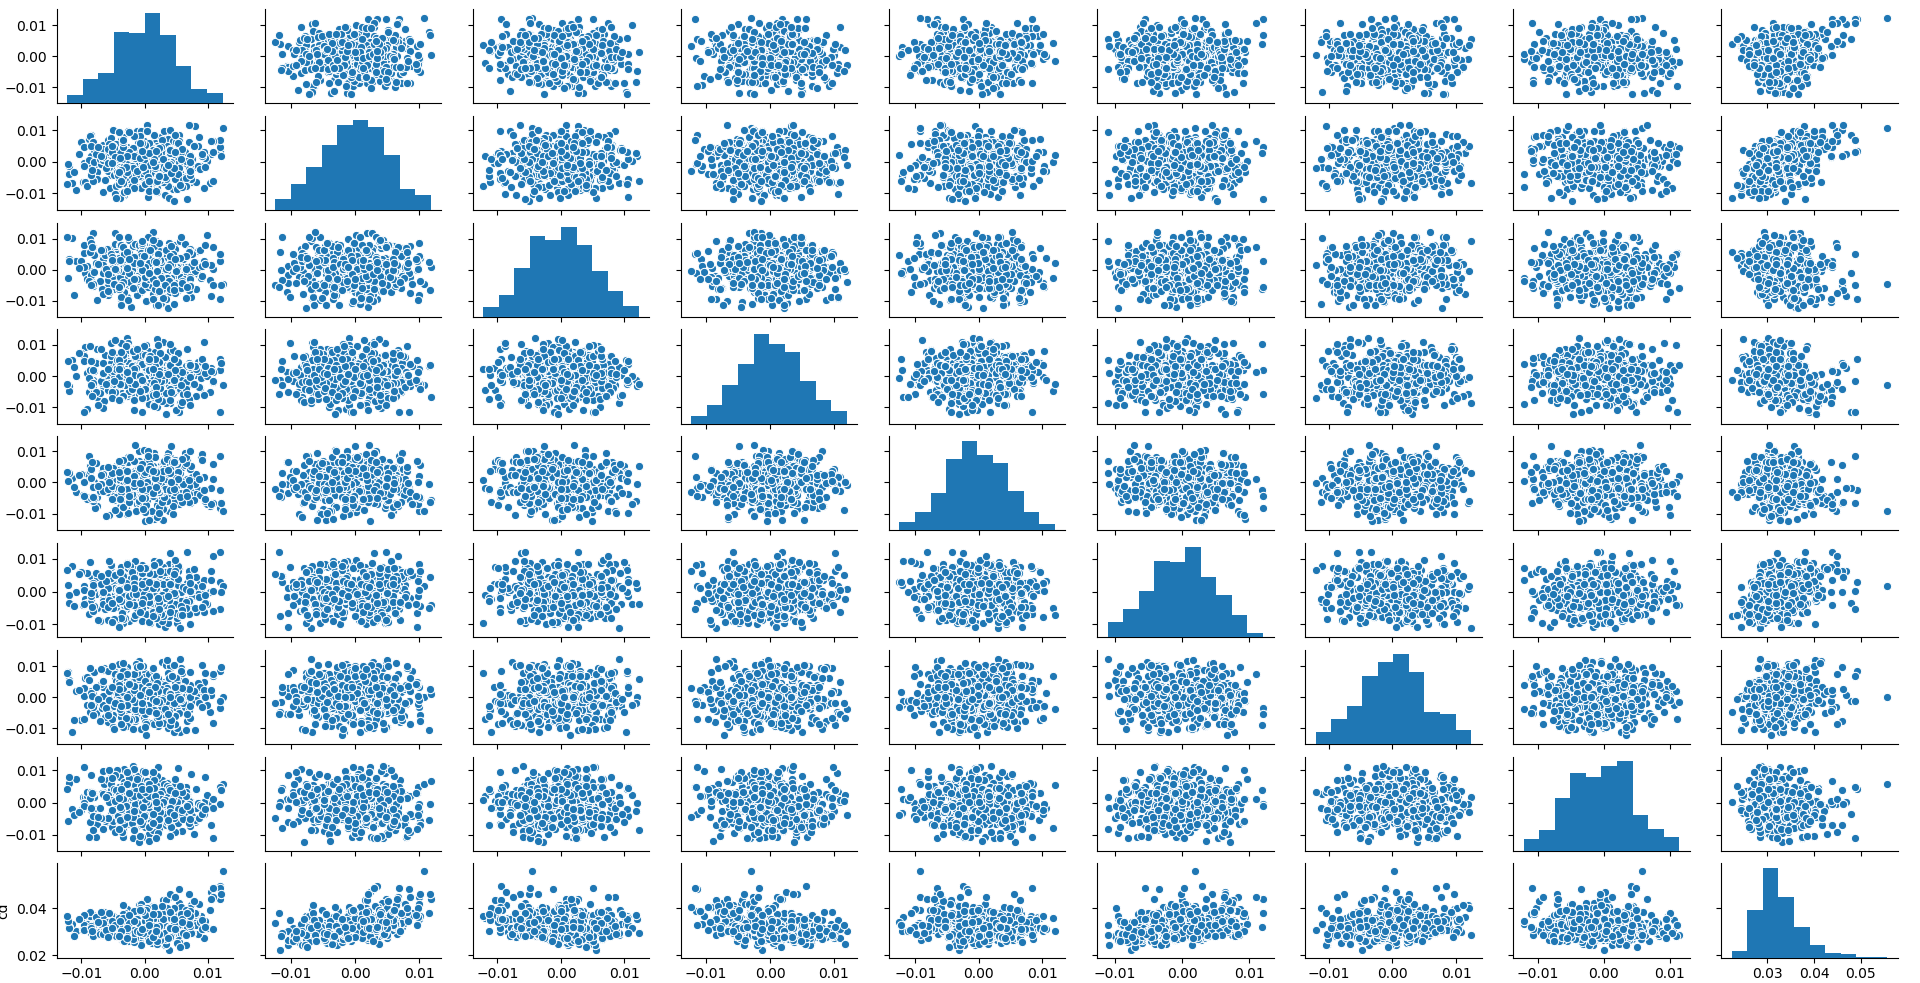
\includegraphics[width=1.0\textwidth,
				trim=0.25cm 0.25cm 0.25cm 0.25cm,
				clip]{figures/single_8D_dist.png}} 
		 }
		\caption{Scatter plot matrix of the 8D data set}
		\label{scatter}
	\end{center}
\end{figure}



\section{Approach}
In this project report, we used the following approach;
\begin{enumerate}
    \item Divide the data into training and truth sets (80-20 plan).
    \item Draw out samples using Halton sequence ($N_s${ = 60}) from the training set.
    \item Train the model.
    \item Predict using truth set inputs.
    \item Estimate model performance using different metrics.
\end{enumerate}

For performance measurement, the following metrics are used;
\begin{itemize}
    \item Normalized root mean square, NRMSE (\%)
    \begin{equation}
\label{nrmse}
		NRMSE = 100 * \sqrt{\frac{1}{m}\sum_{i}^{m}\left(\frac{y_i - \hat{y_i}}{y_i}\right)^2}
		\end{equation}
    
    \item Coefficient of determination, R2 score, $R^2$
        \begin{equation}
		R^2  =  1- \frac{\sum_{i}^{m}\left(y_i - \hat{y_i}\right)^2}{\sum_{i}^{m}\left(y_i - \bar{y}\right)^2}
		\end{equation}
\end{itemize}
where m is the number of test points (truth set), $y_i$ is the output of the truth set,  $\hat{y_i}$ is the predicted result and \bar{y_i} is the mean of output of the truth set for every i-point.


\section{The Halton-based sampling plan}
Sampling points used for model training are crucial in the performance of Kriging-based models. It is desirable to have sample data that best describes the given dataset else, the model might have overfitting problems. Because of this, the choice of sampling plan for Kriging / Gaussian processes is not a trivial task. To better improve efficiency of our models, we developed a Halton-based sampling plan to achieve uniformity of data distributions. The algorithm is shown below;
    \begin{algorithm}[H]
\DontPrintSemicolon
  
  \KwInput{Sampling size, $N_s$}
  \KwOutput{{$x_{sample}$,$y_{sample}$}}
  \KwData{$\mathbf{x},y$}
  Get k from the data\\
  Design a Halton sequence with dimension,k and size,$N_s$\\
  Normalize $\mathbf{x}$ : $x_{norm}$\\
  Map the generated sequence on $x_{norm}$ and select the  nearest points: $x_{s,norm}$\\
  Denormalize $x_{s,norm}$ : $x_{sample}$\\
  Get the corresponding data from y : $y_{sample}$
% \caption{Example code}
\end{algorithm}

Figure \ref{fig:halton} shows the robustness of our developed sampling plan in drawing sampling that best represent the whole dataset.

\begin{figure}[!h]
	\begin{center}
		\vspace{-10pt}
		\mbox{ \subfloat[Data]{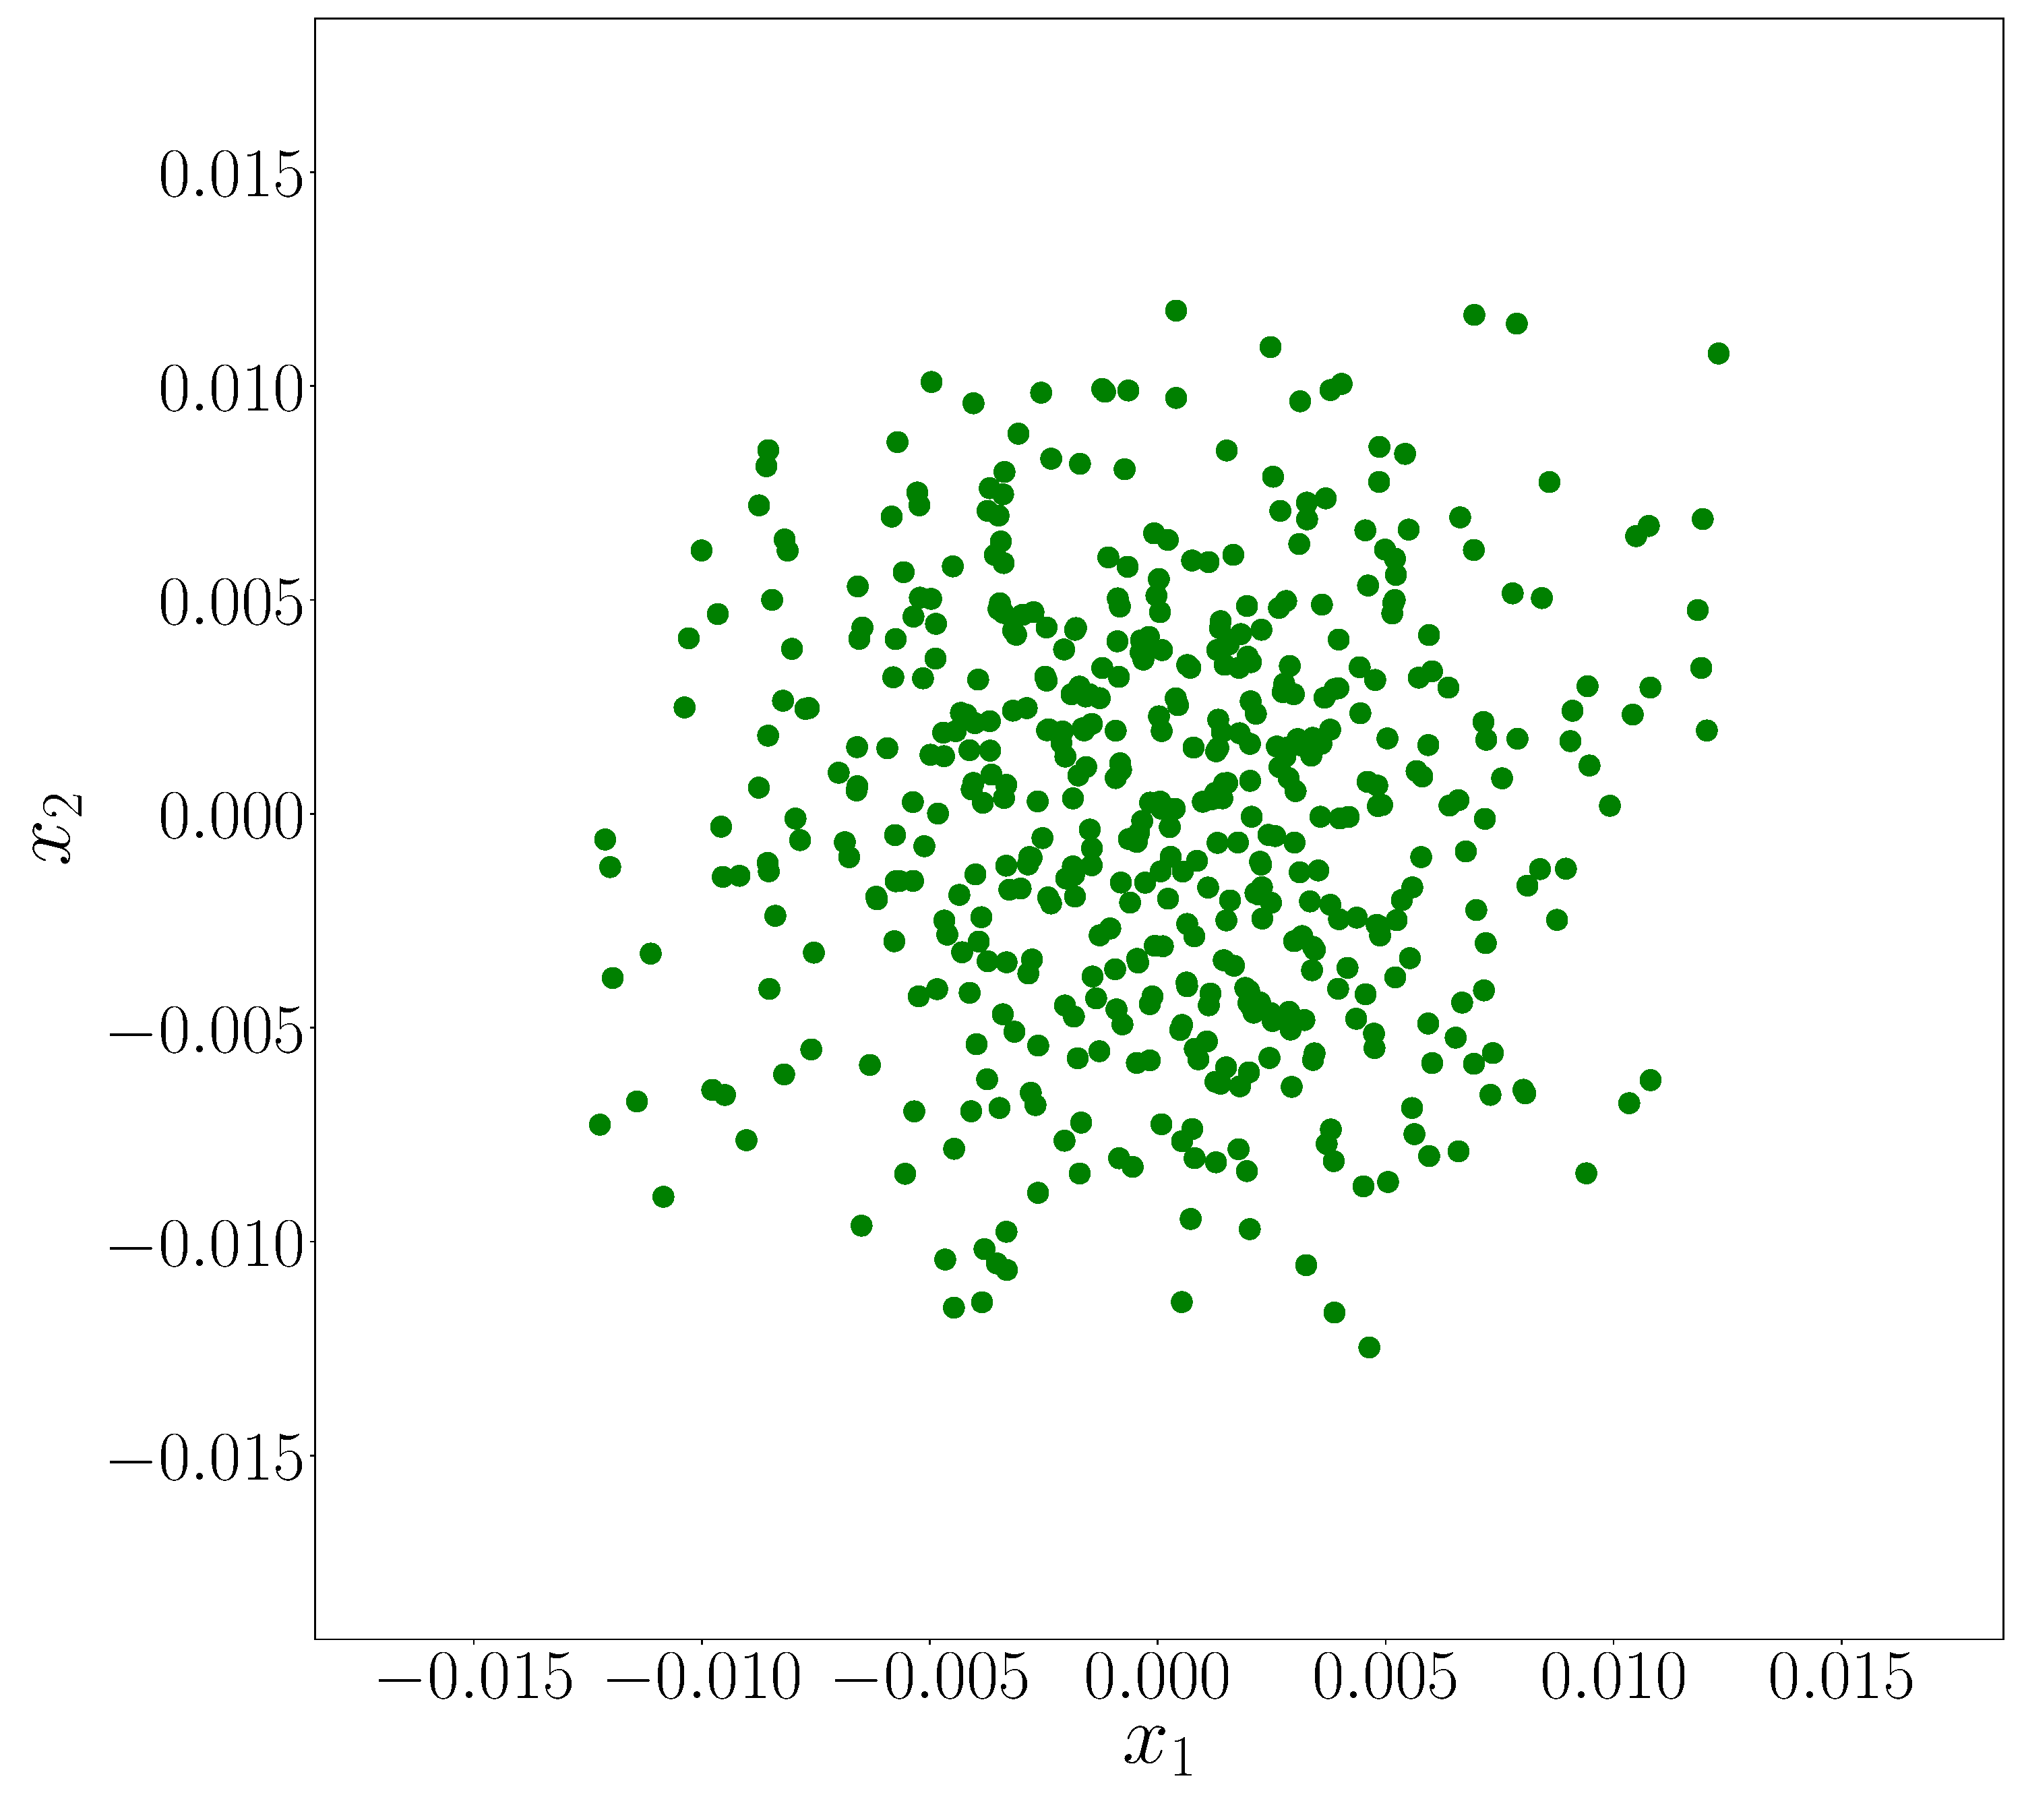
\includegraphics[width=0.50\textwidth,
				trim=0.25cm 0.25cm 0.25cm 0.25cm,
				clip]{figures/single_2D.pdf}} 
			\subfloat[Samples (100)]{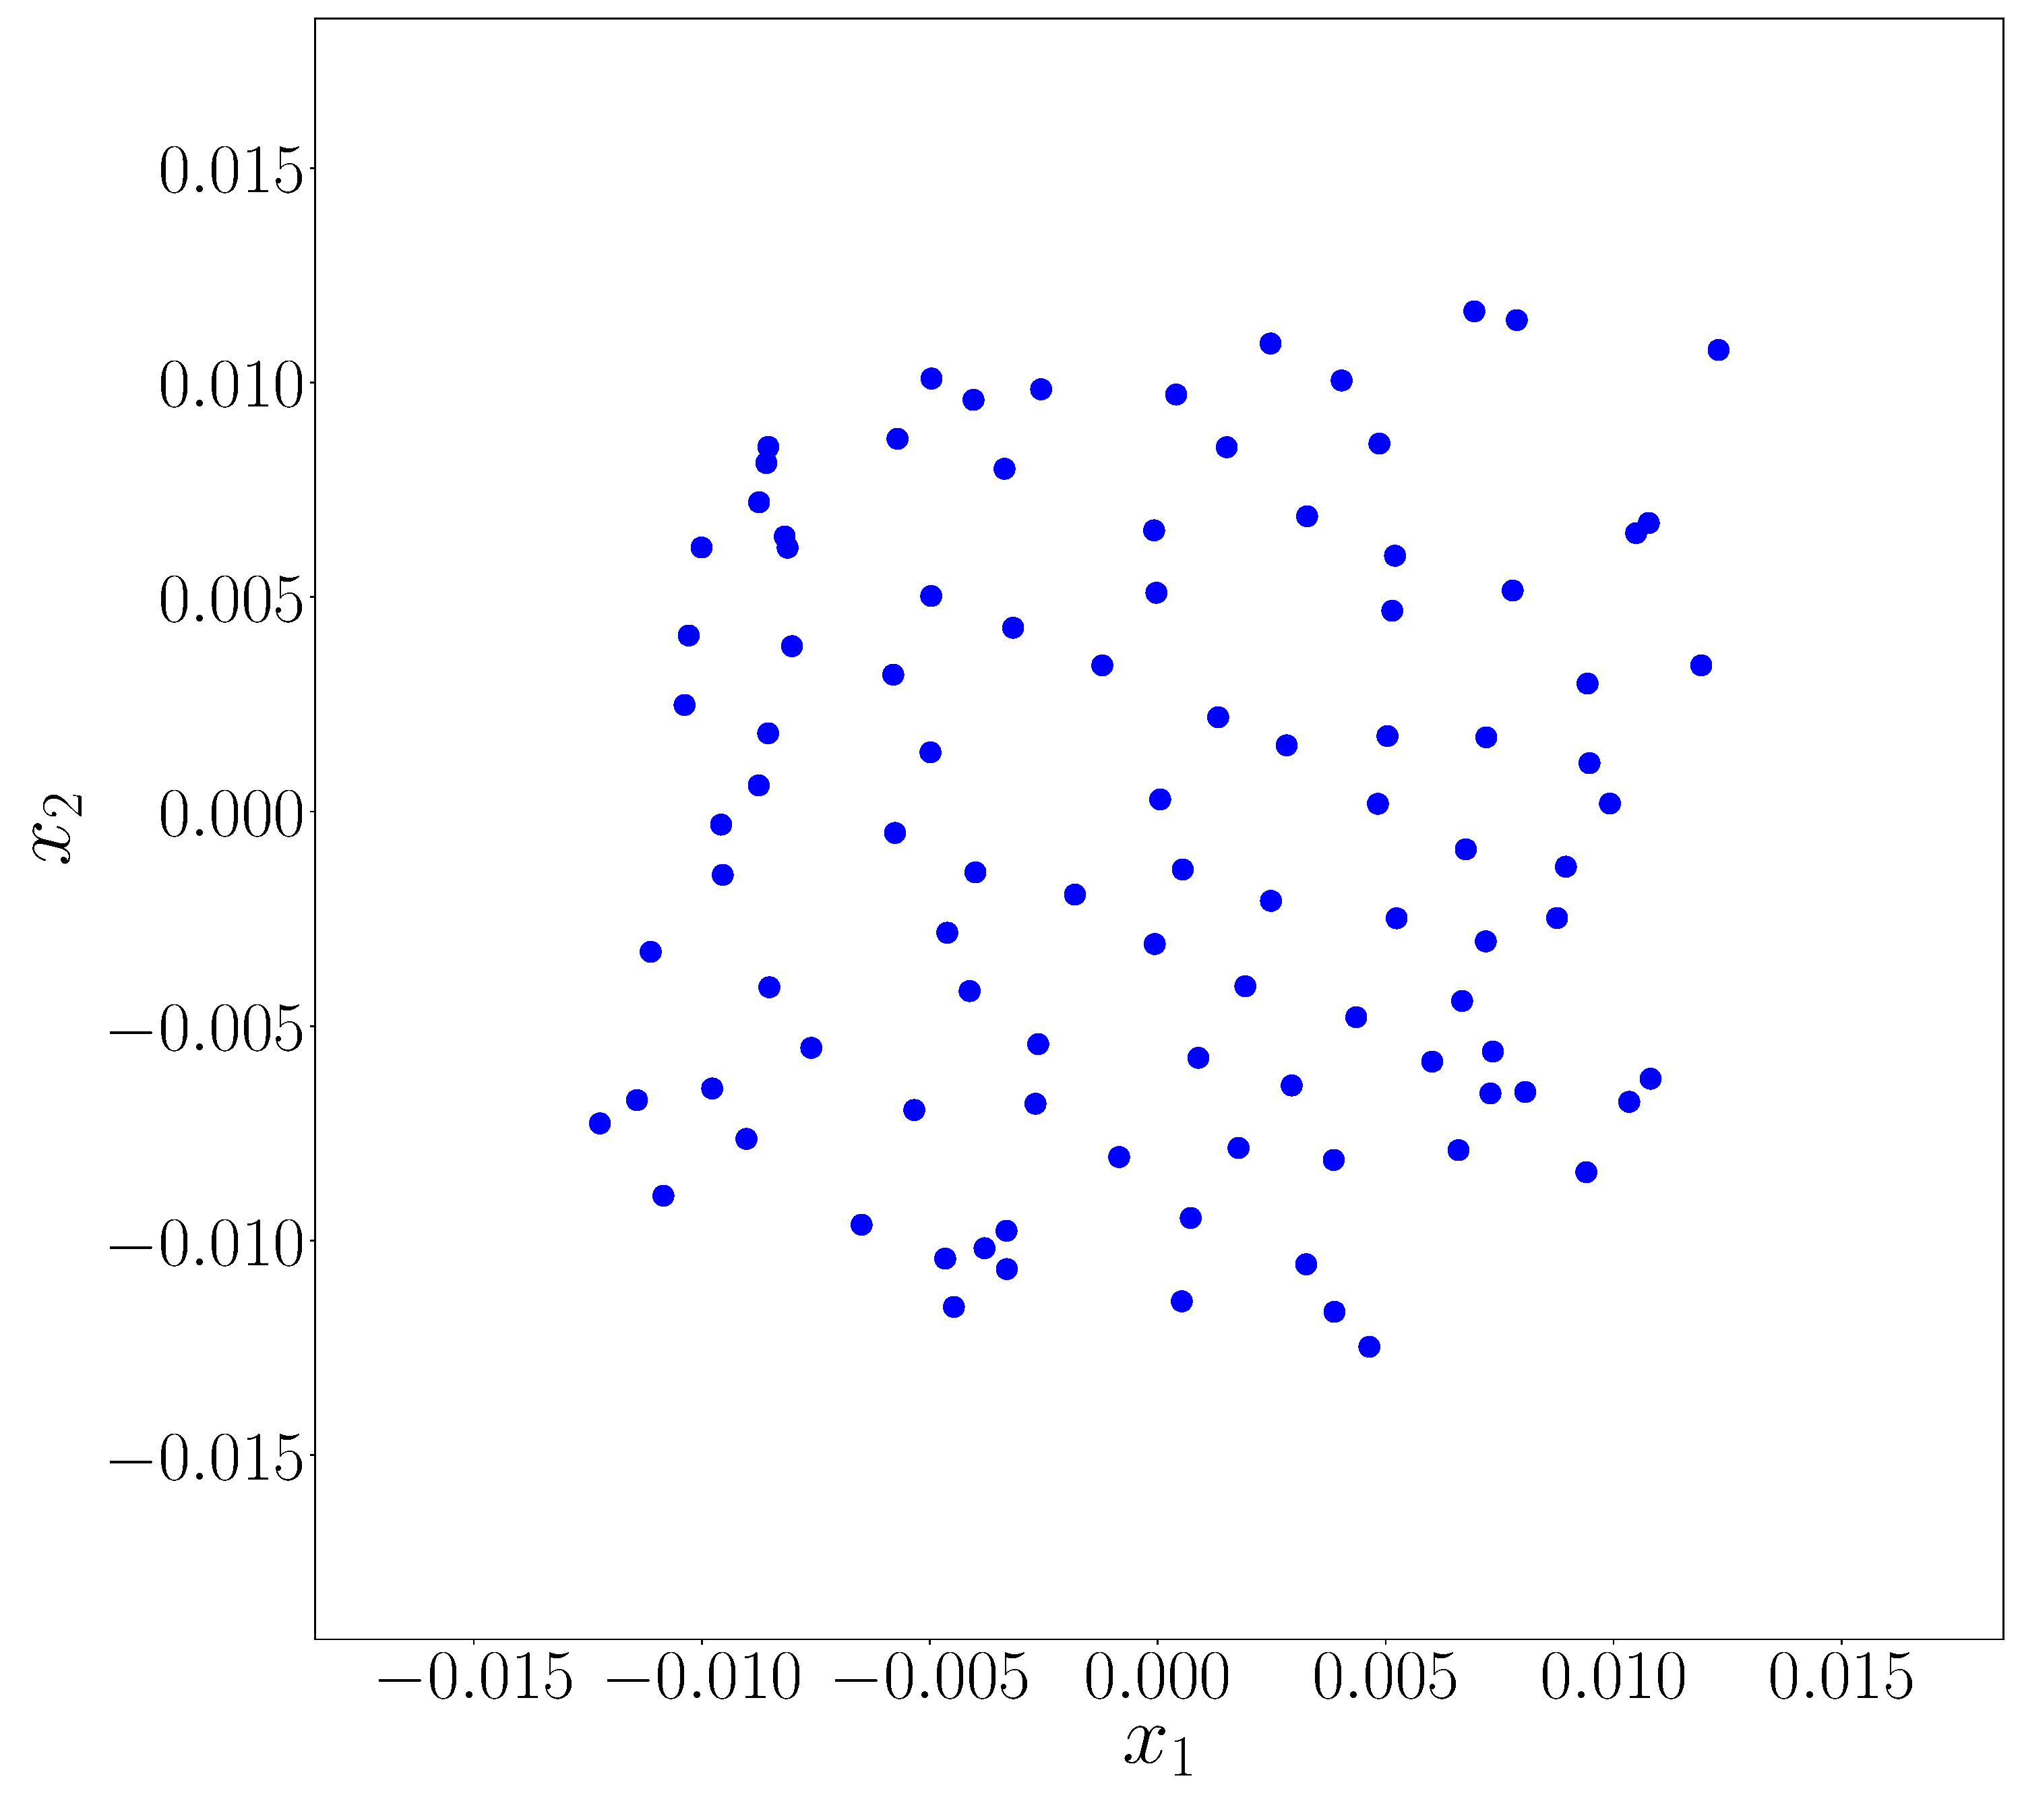
\includegraphics[width=0.50\textwidth,
				trim=0.25cm 0.25cm 0.25cm 0.25cm,
				clip]{figures/single_2D_sample.pdf}} }
		\caption{An illustration of the sampling distribution}
		\label{fig:halton}
	\end{center}
\end{figure}

\section{Results}
Using the seven models, we bechmarked their performance on the 8D and 16D datasets and also checked the contributions of the single kernels in the multiple kernel methods. Figure \ref{fig:ensemble_weights} and \ref{fig:ckl_weights} show the contributions of the four individual kernels in the ensemble and CKL methods respectively. From the weighting achieved in the ensemble models, the predominance of the Mat\'ern kernels (3/2 and 5/2) is seen in both 8D and 16D data sets. Similarly, the Gaussian and Mat\'ern 5/2 kernels are more predominant in the CKL formulations. The performance metric of the models are summarized in Figures \ref{fig:nrmse} and \ref{fig:r2_score}. The NRMSE metric is more appropriate for the model comparison. It shows that the MCKL model performed best followed by the CKL model in both benchmarkings. However, the training times shown in Figure \ref{fig:training_time} reveals the high computational time required by the MCKL model. 
\begin{figure}[!h]
	\begin{center}
		\vspace{-10pt}
		\mbox{ \subfloat[8D]{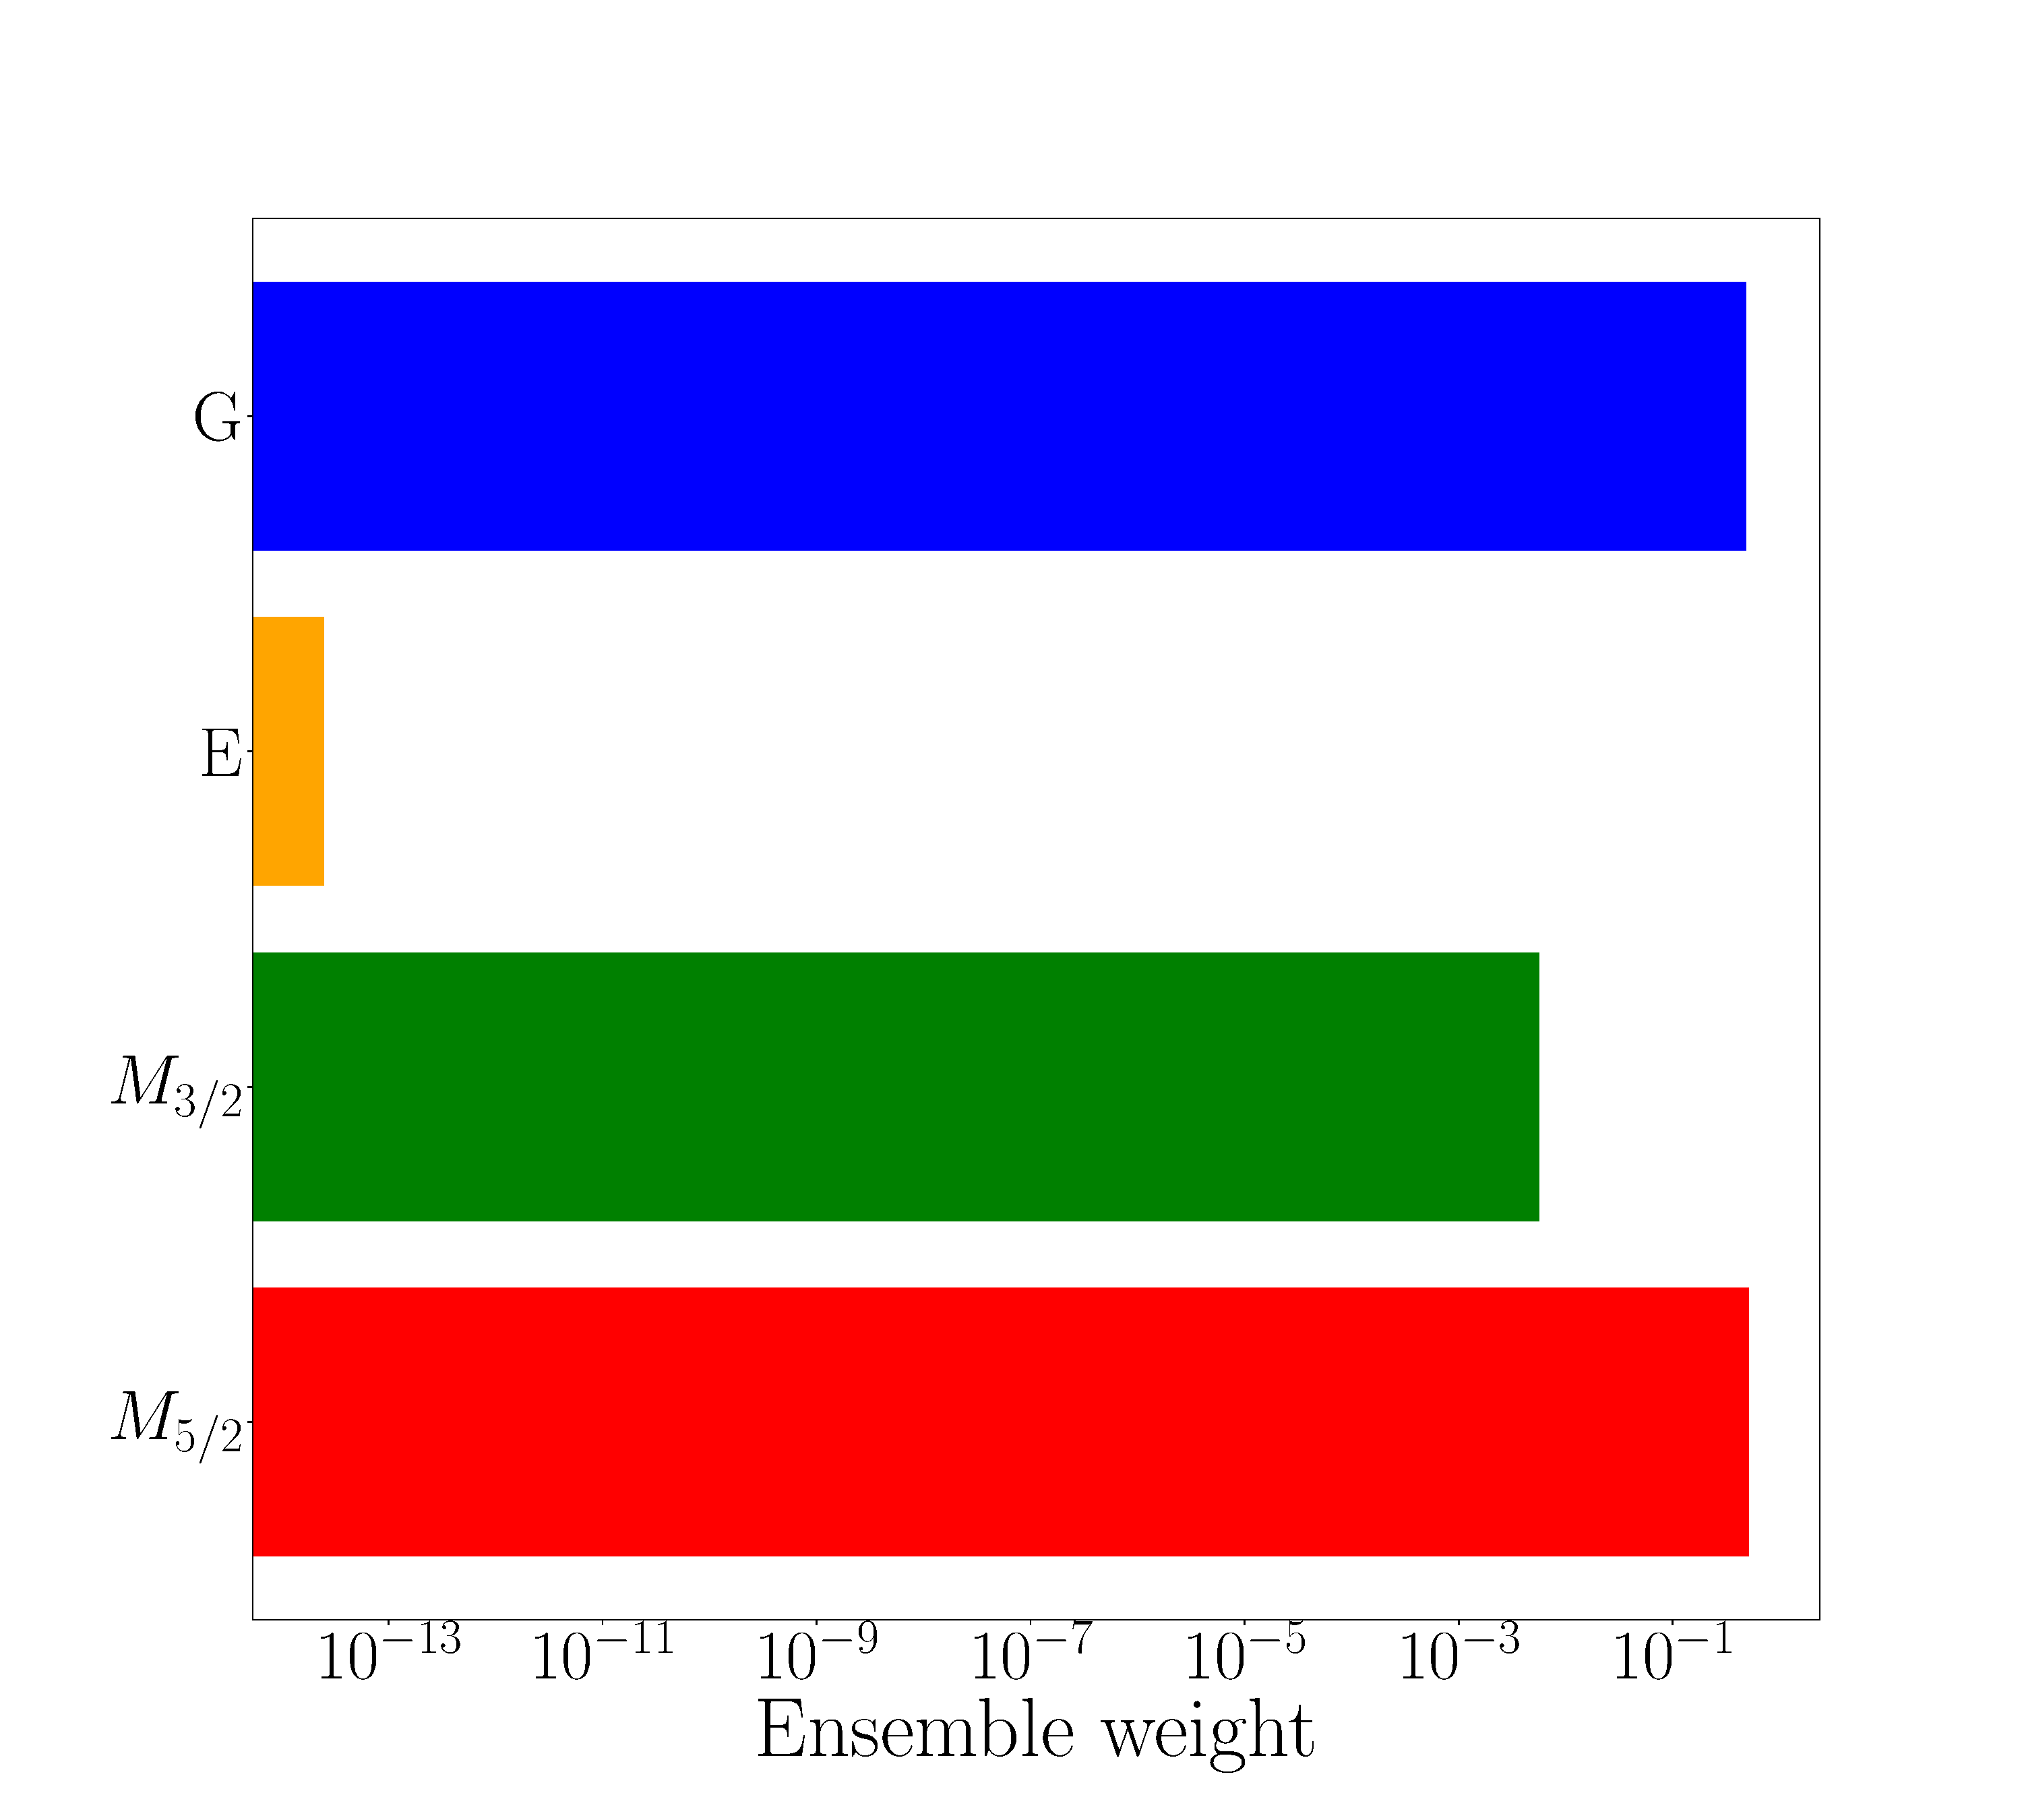
\includegraphics[width=0.50\textwidth,
				trim=0.25cm 0.25cm 0.25cm 0.25cm,
				clip]{figures/single_8D_ensemble_weight.pdf}} 
			\subfloat[16D]{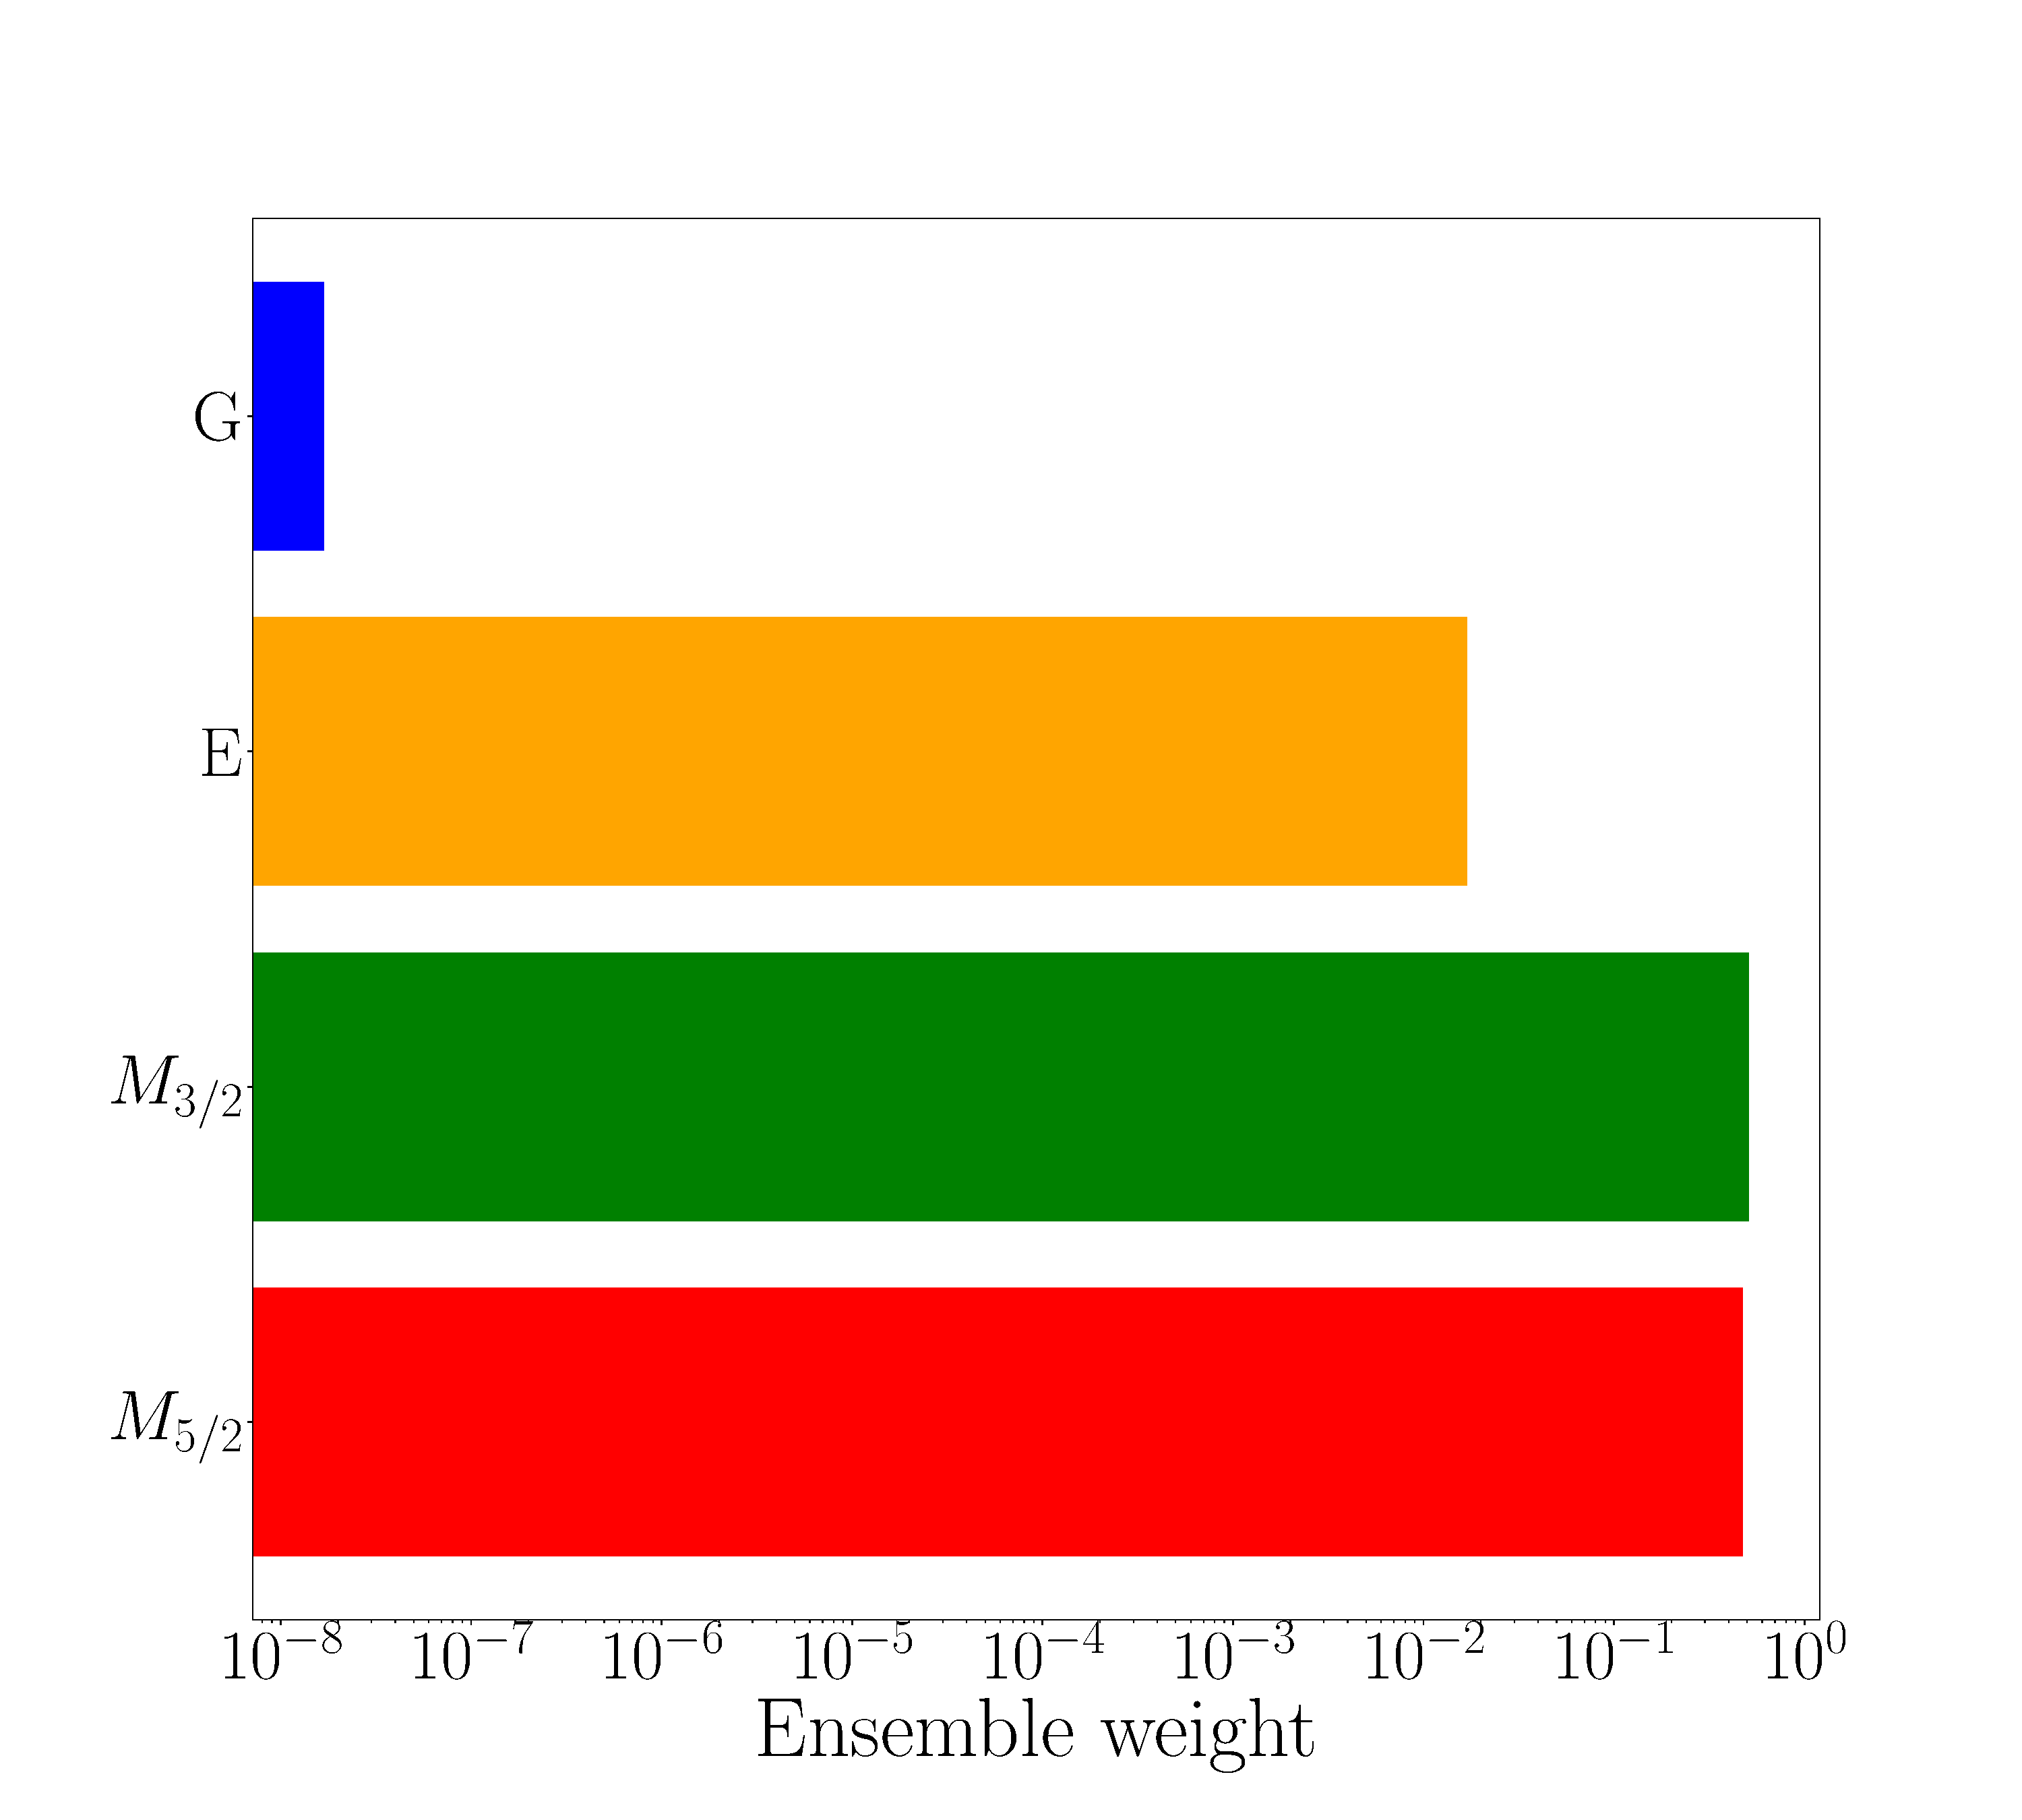
\includegraphics[width=0.50\textwidth,
				trim=0.25cm 0.25cm 0.25cm 0.25cm,
				clip]{figures/single_16D_ensemble_weight.pdf}} }
		\caption{Ensemble weights}
		\label{fig:ensemble_weights}
	\end{center}
\end{figure}


\begin{figure}[!h]
	\begin{center}
		\vspace{-10pt}
		\mbox{ \subfloat[8D]{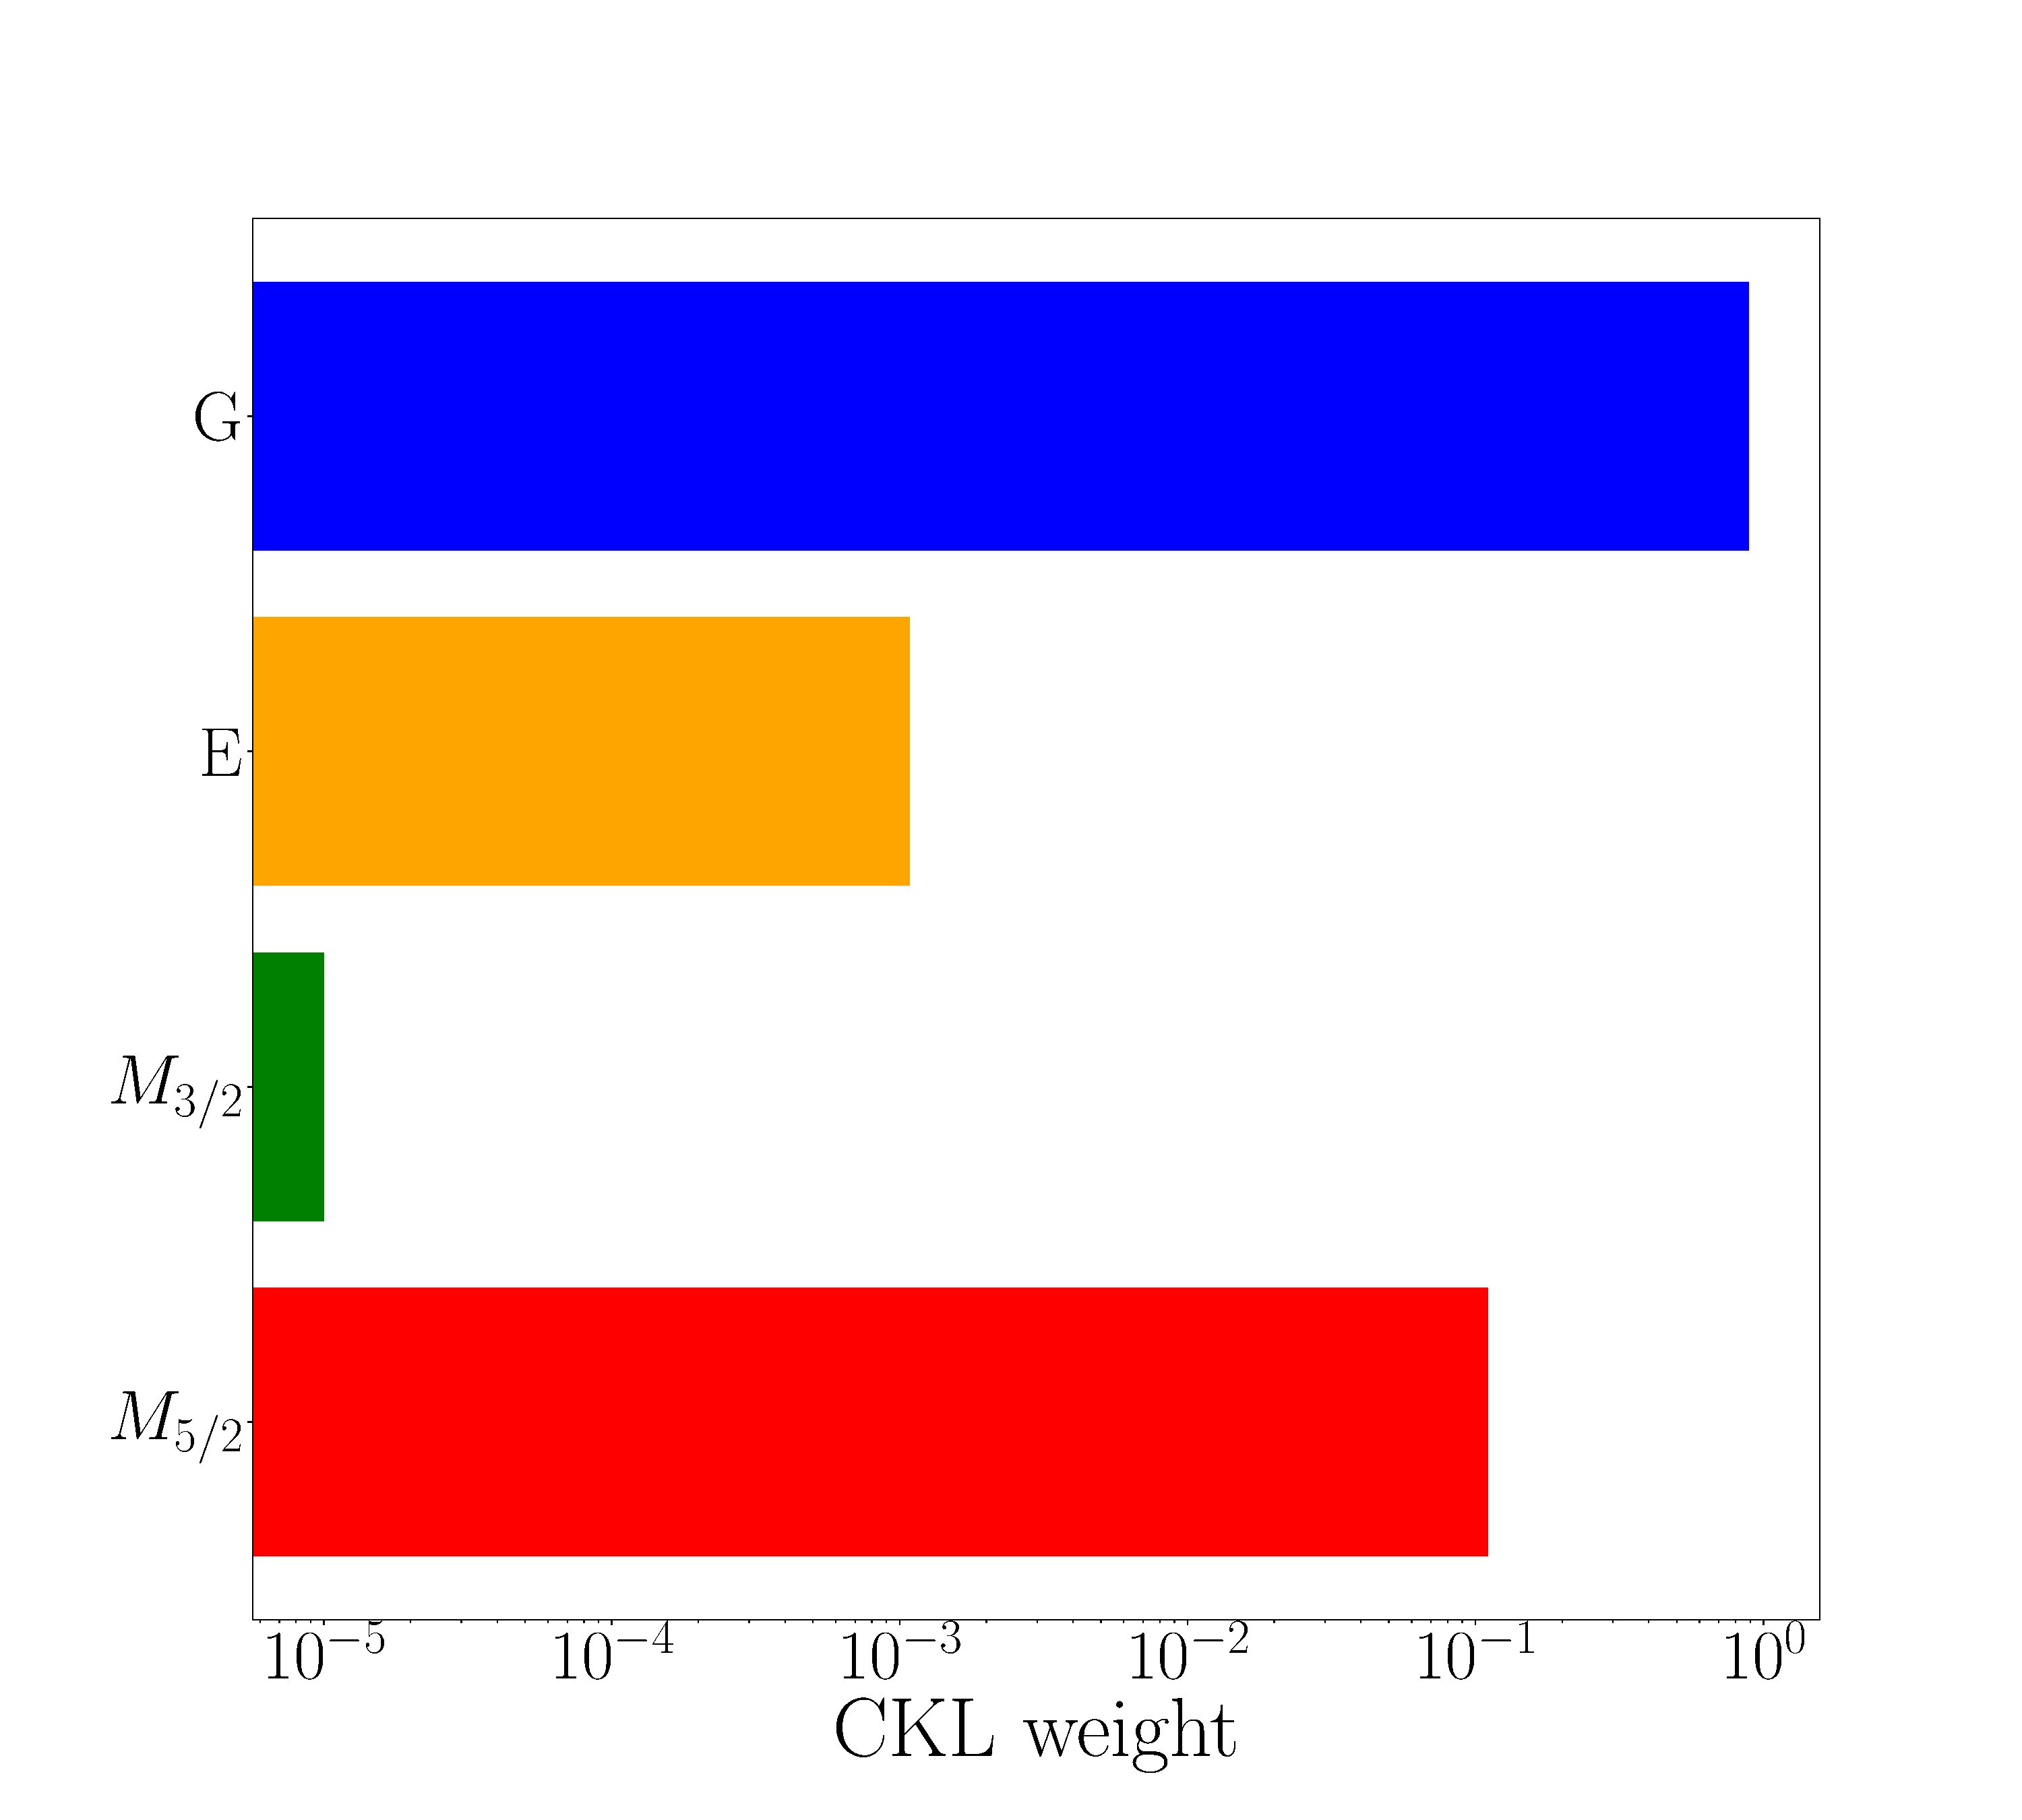
\includegraphics[width=0.50\textwidth,
				trim=0.25cm 0.25cm 0.25cm 0.25cm,
				clip]{figures/single_8D_ckl_weight.pdf}} 
			\subfloat[16D]{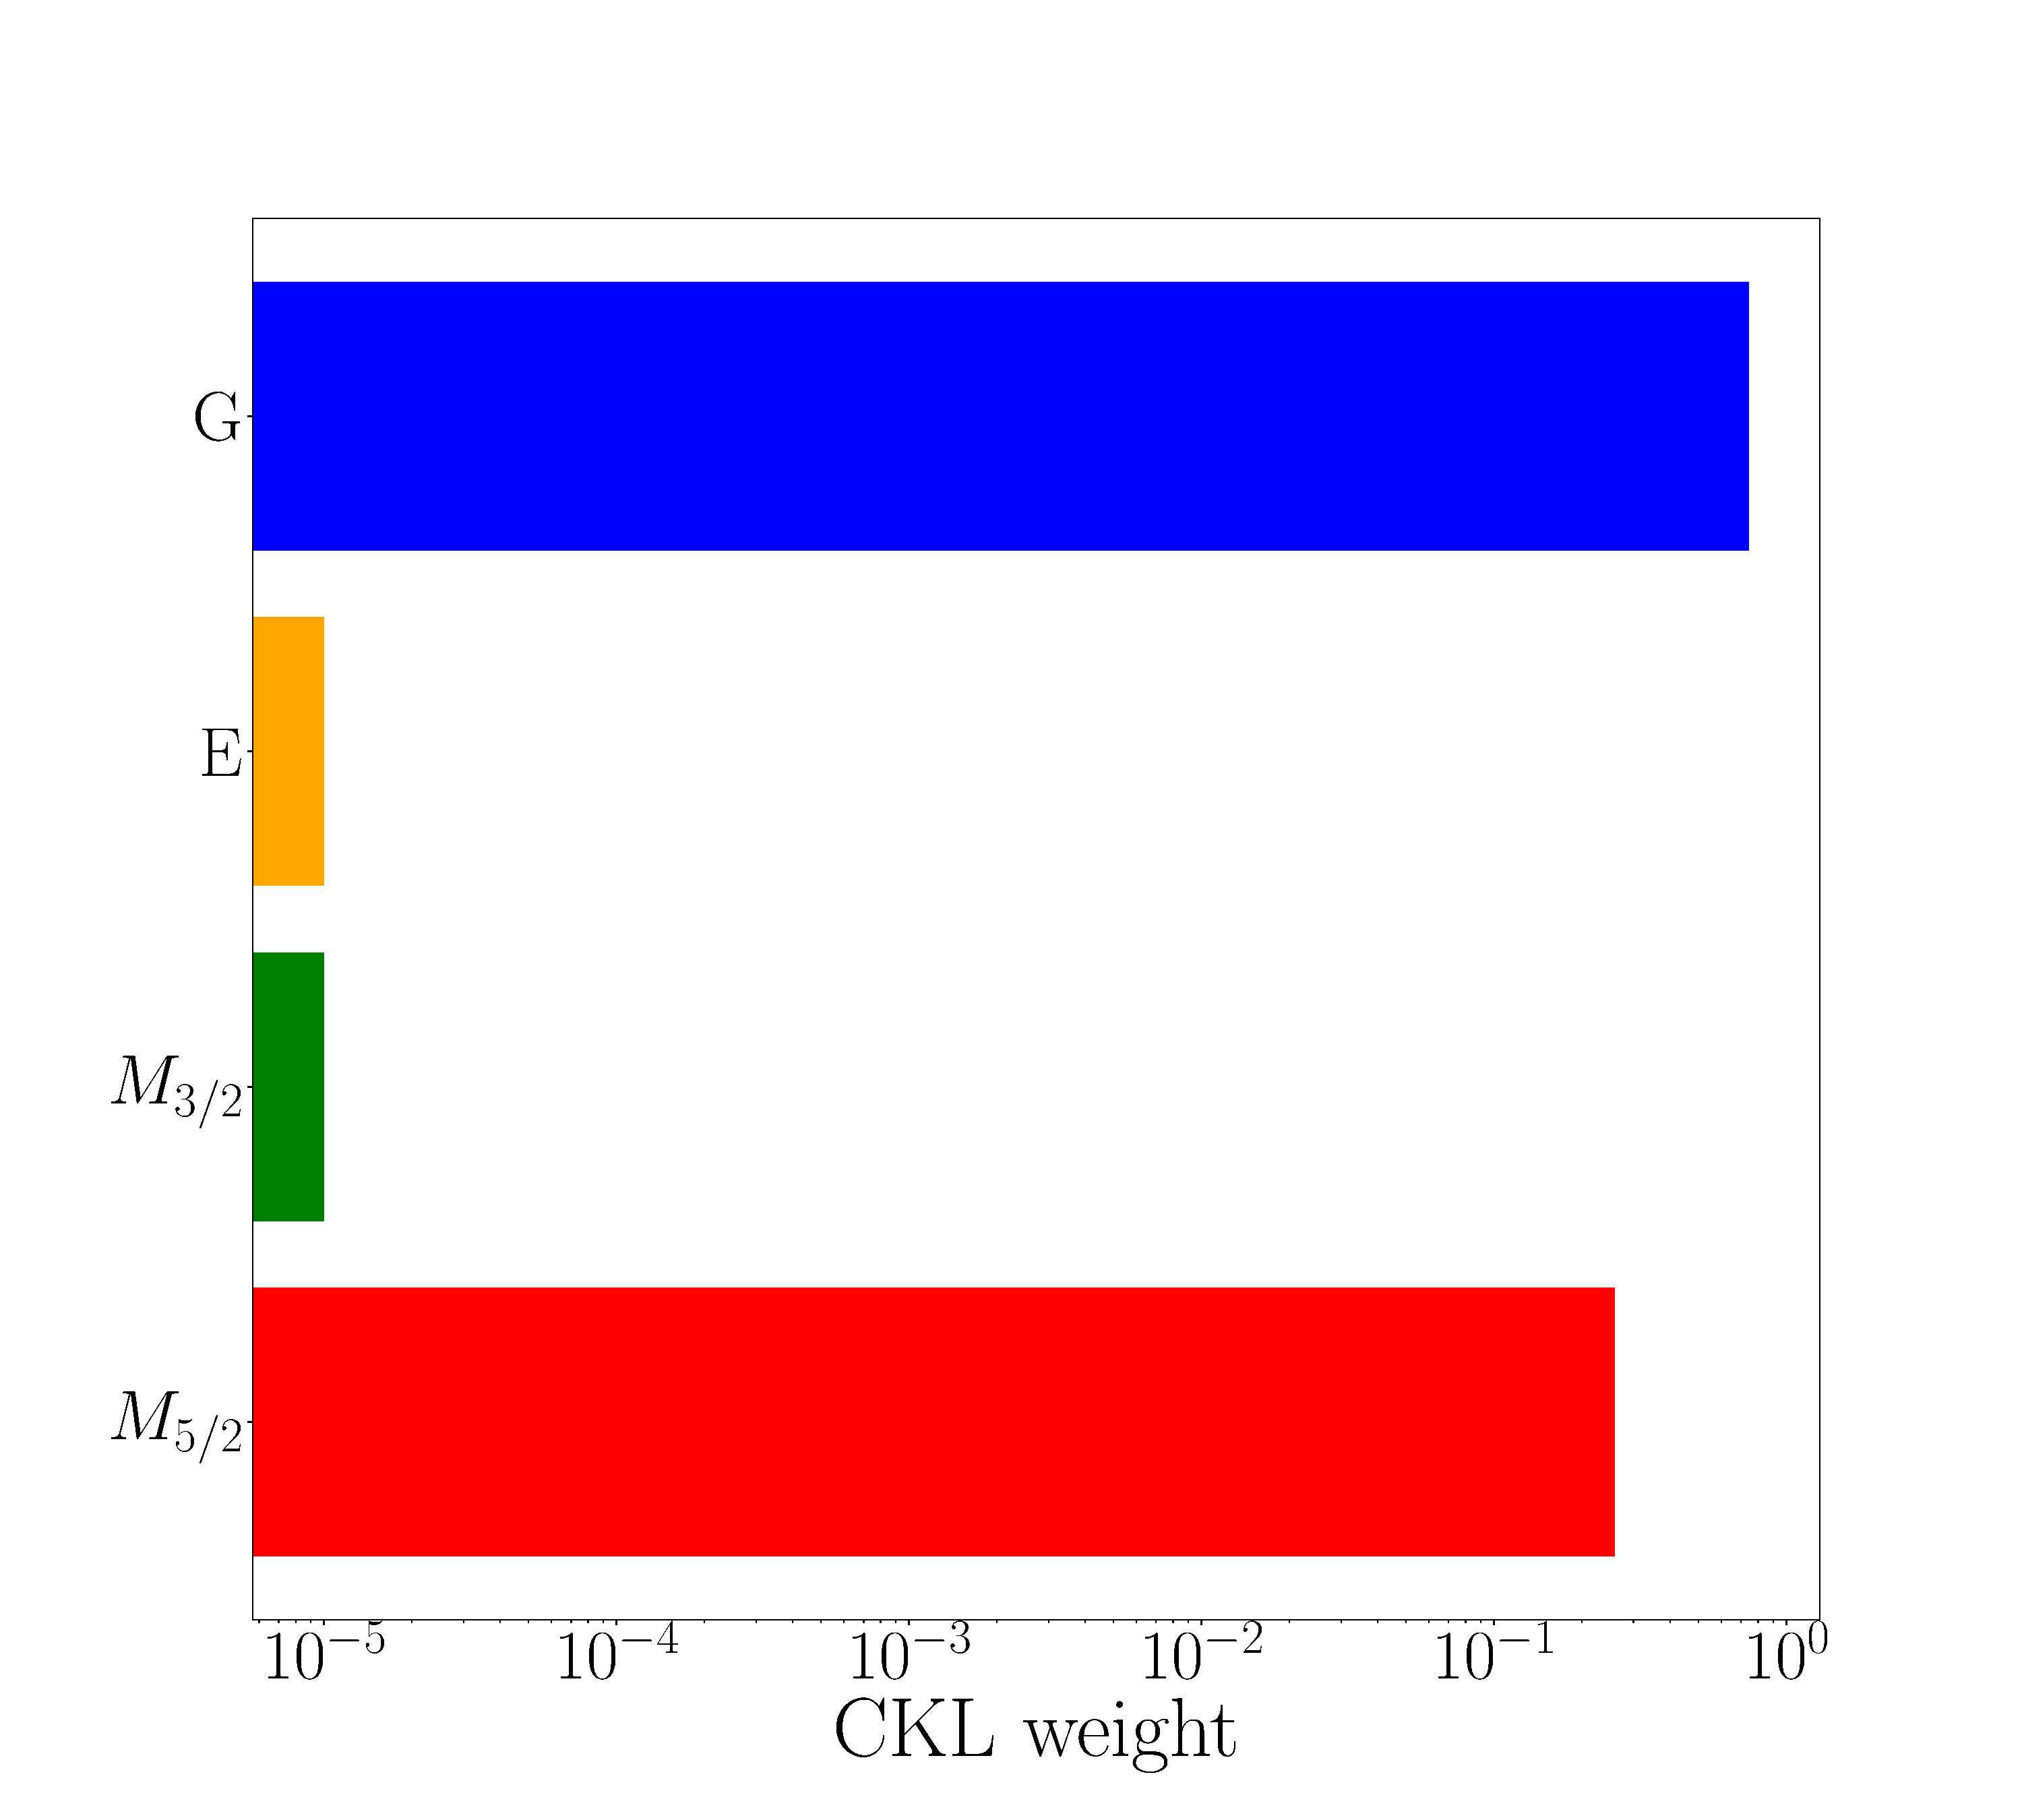
\includegraphics[width=0.50\textwidth,
				trim=0.25cm 0.25cm 0.25cm 0.25cm,
				clip]{figures/single_16D_ckl_weight.pdf}} }
		\caption{CKL weights}
		\label{fig:ckl_weights}
	\end{center}
\end{figure}


\begin{figure}[!h]
	\begin{center}
		\vspace{-10pt}
		\mbox{ \subfloat[8D]{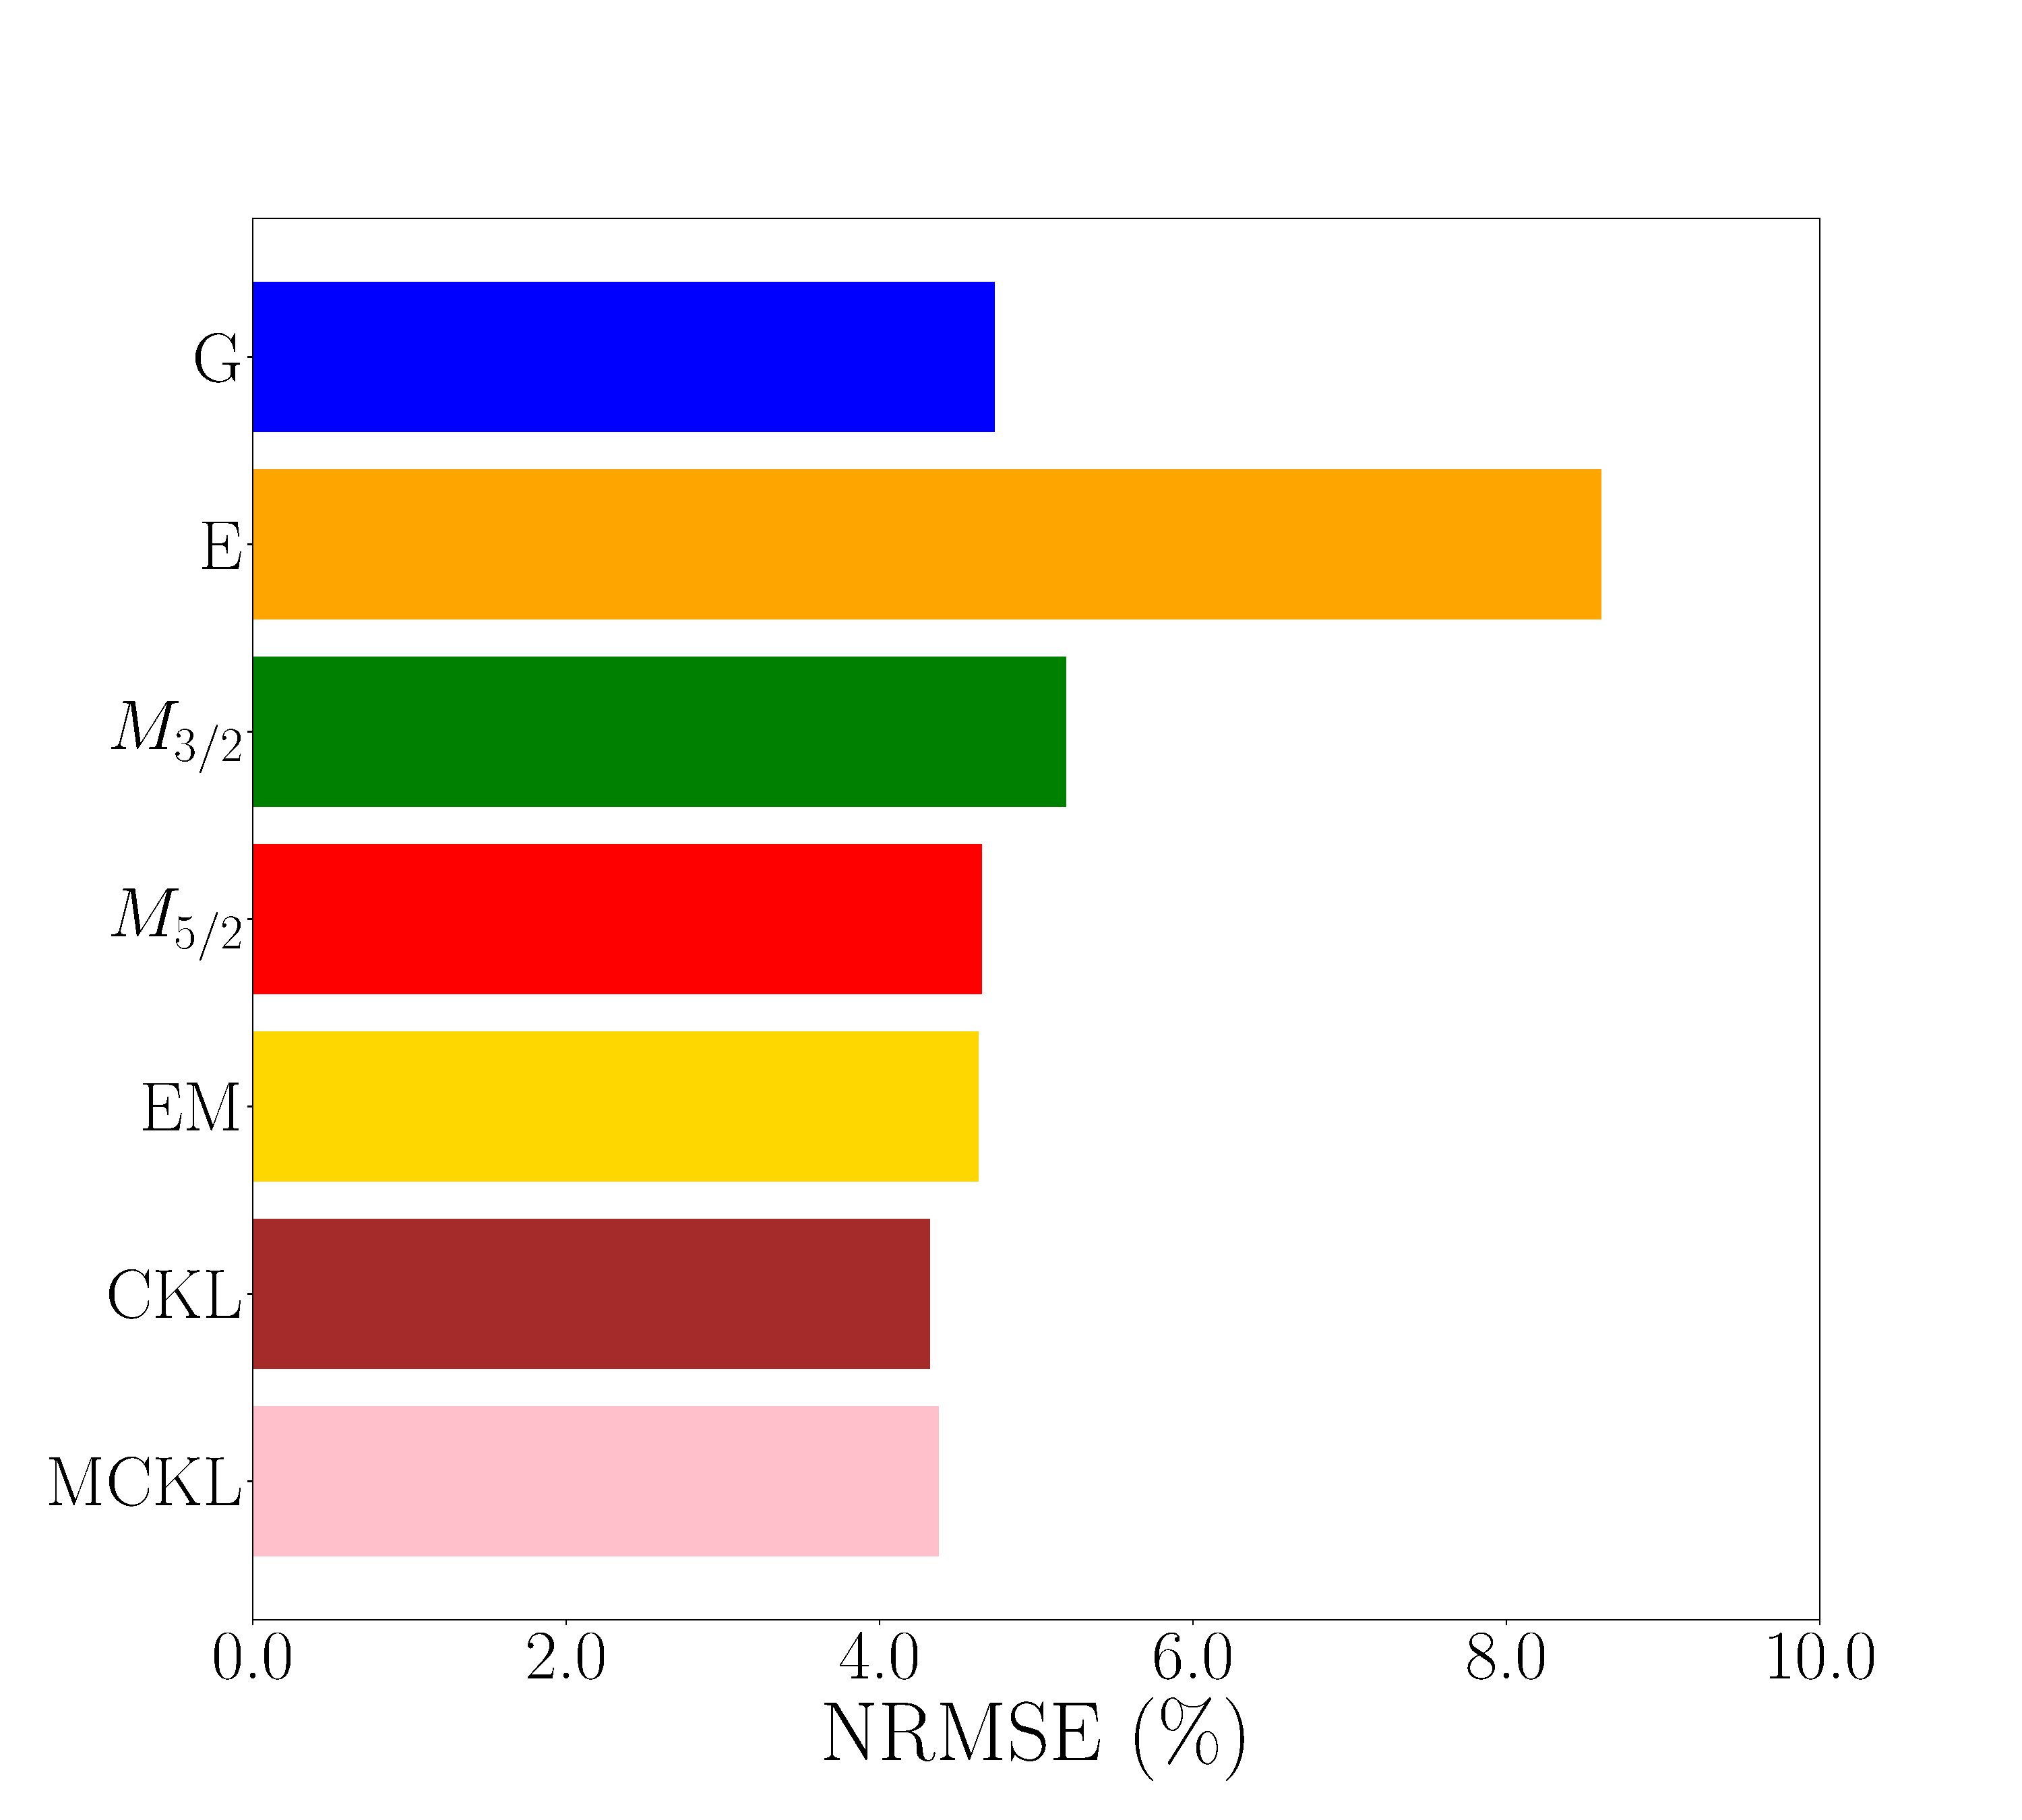
\includegraphics[width=0.50\textwidth,
				trim=0.25cm 0.25cm 0.25cm 0.25cm,
				clip]{figures/single_8D_NRMSE.pdf}} 
			\subfloat[16D]{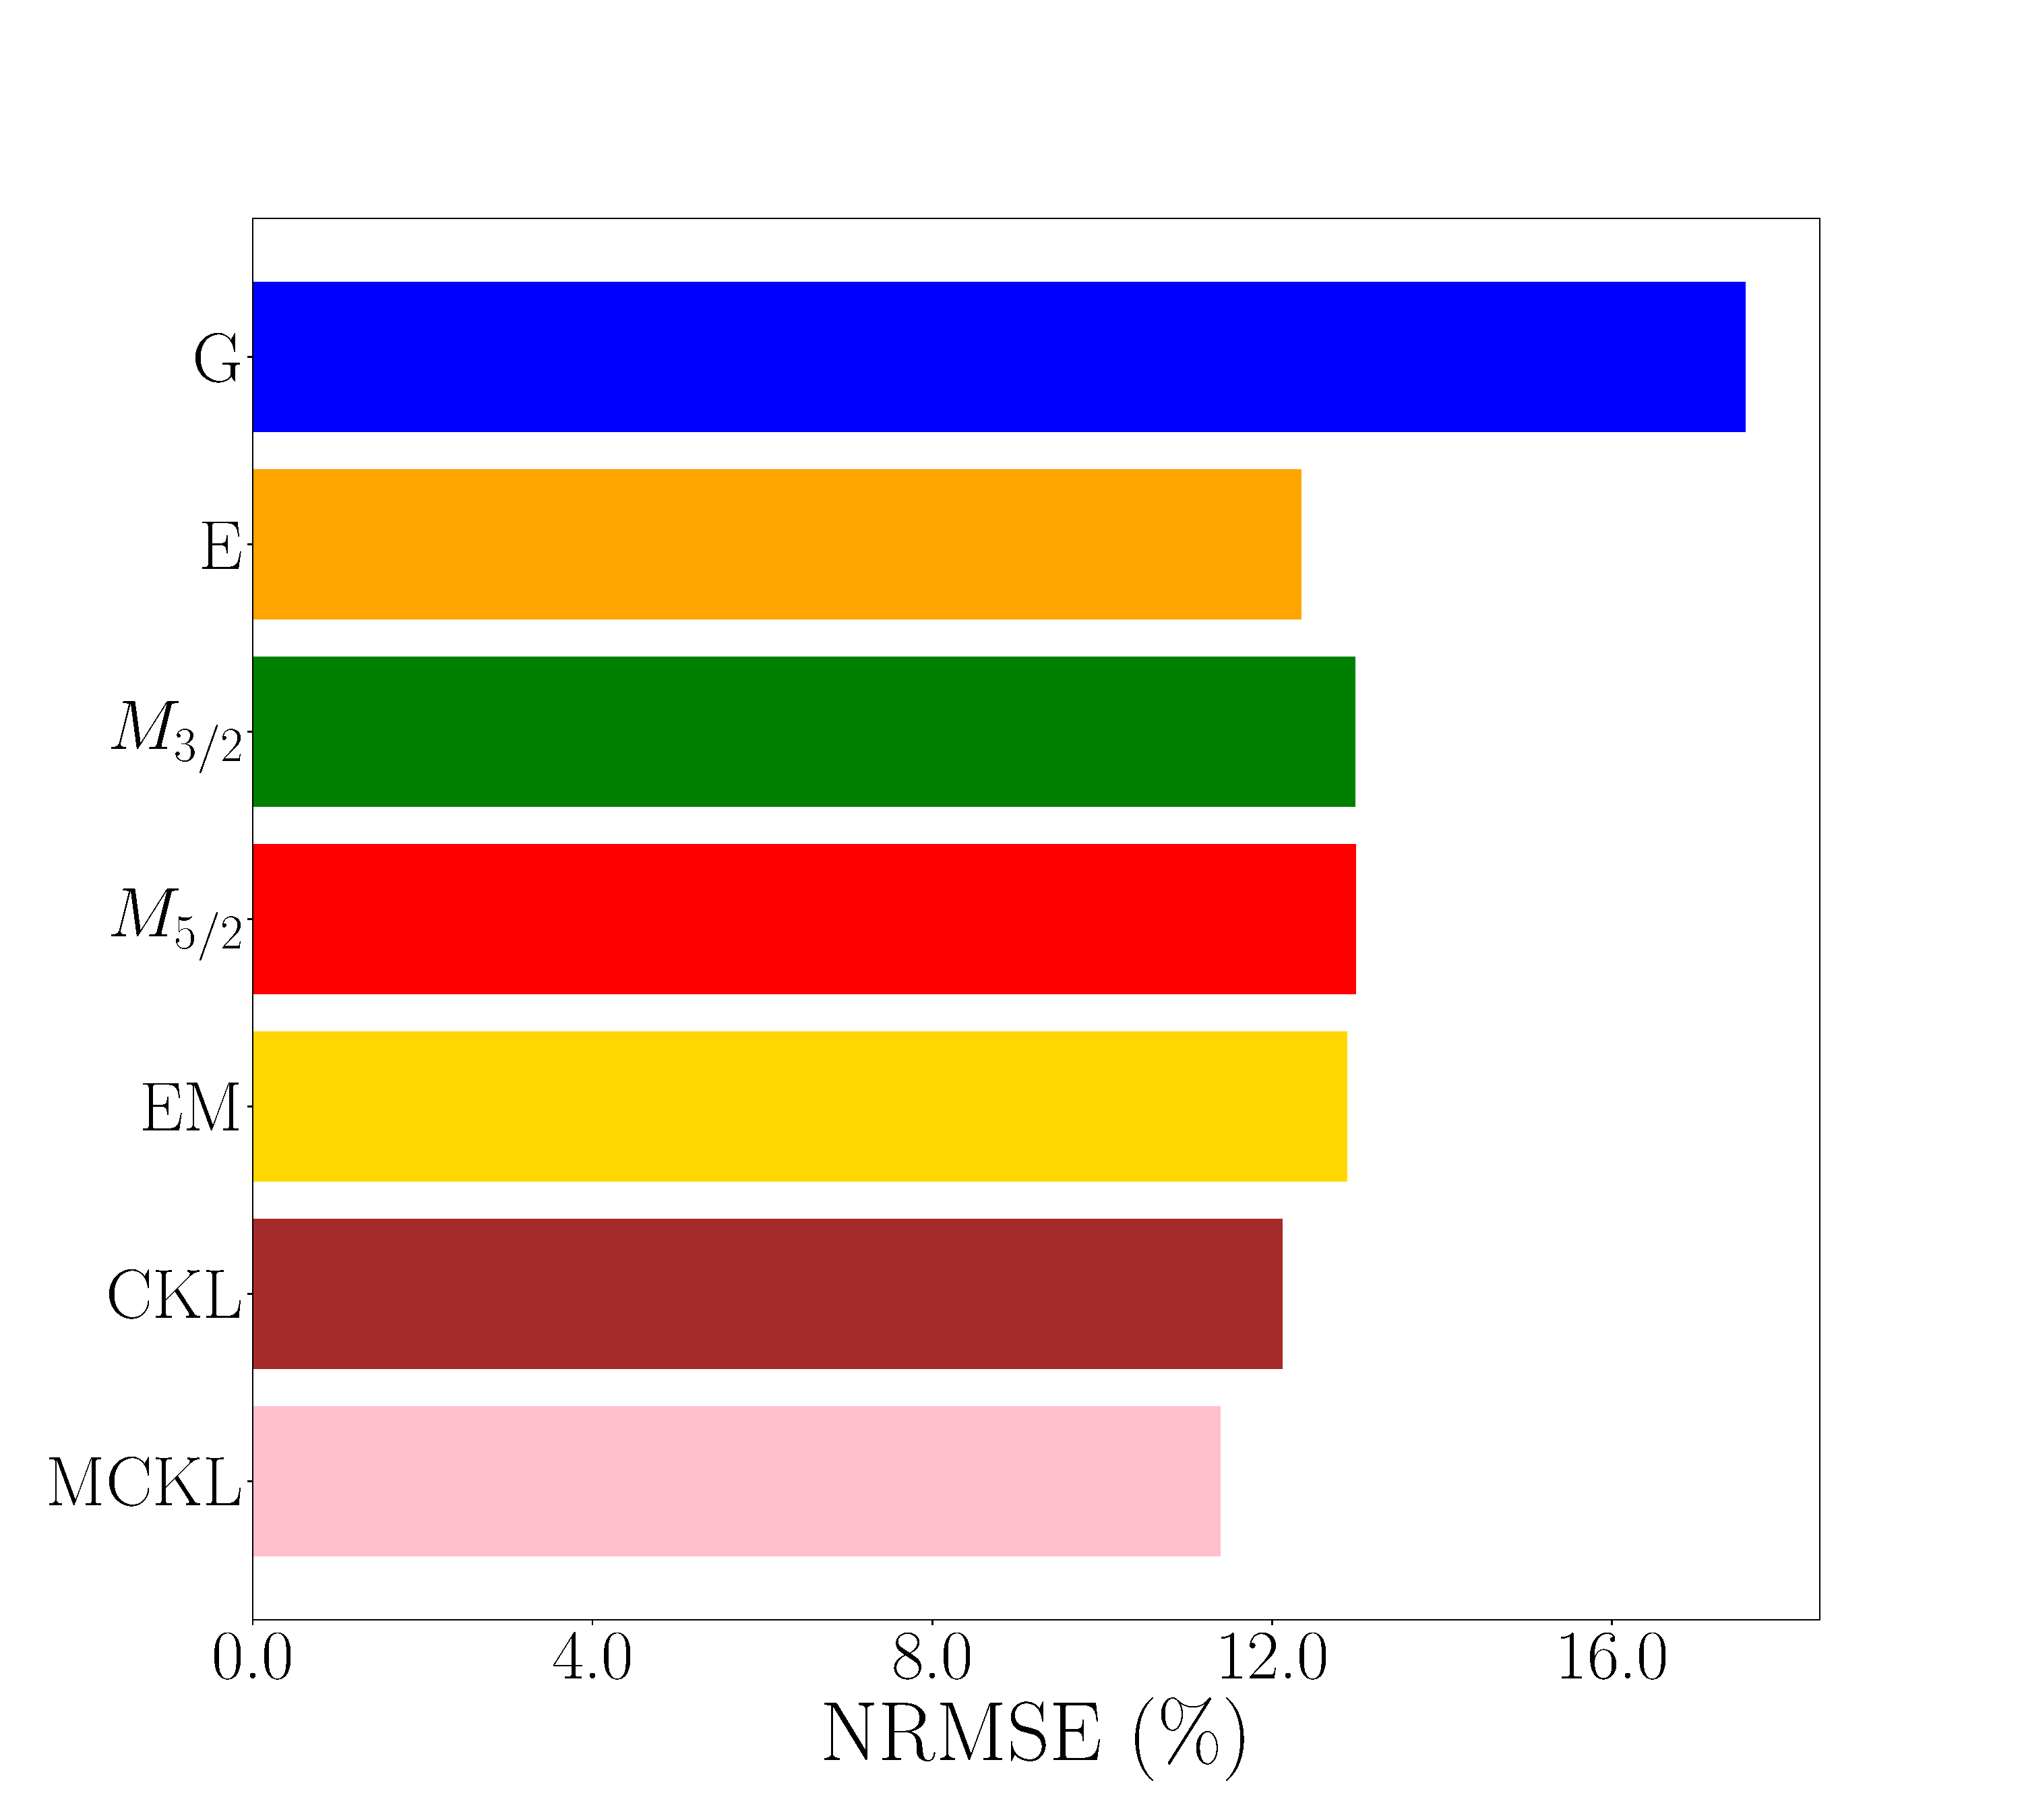
\includegraphics[width=0.50\textwidth,
				trim=0.25cm 0.25cm 0.25cm 0.25cm,
				clip]{figures/single_16D_NRMSE_n.pdf}} }
		\caption{Normalized root mean square errors of predictions}
		\label{fig:nrmse}
	\end{center}
\end{figure}


\begin{figure}[!h]
	\begin{center}
		\vspace{-10pt}
		\mbox{ \subfloat[8D]{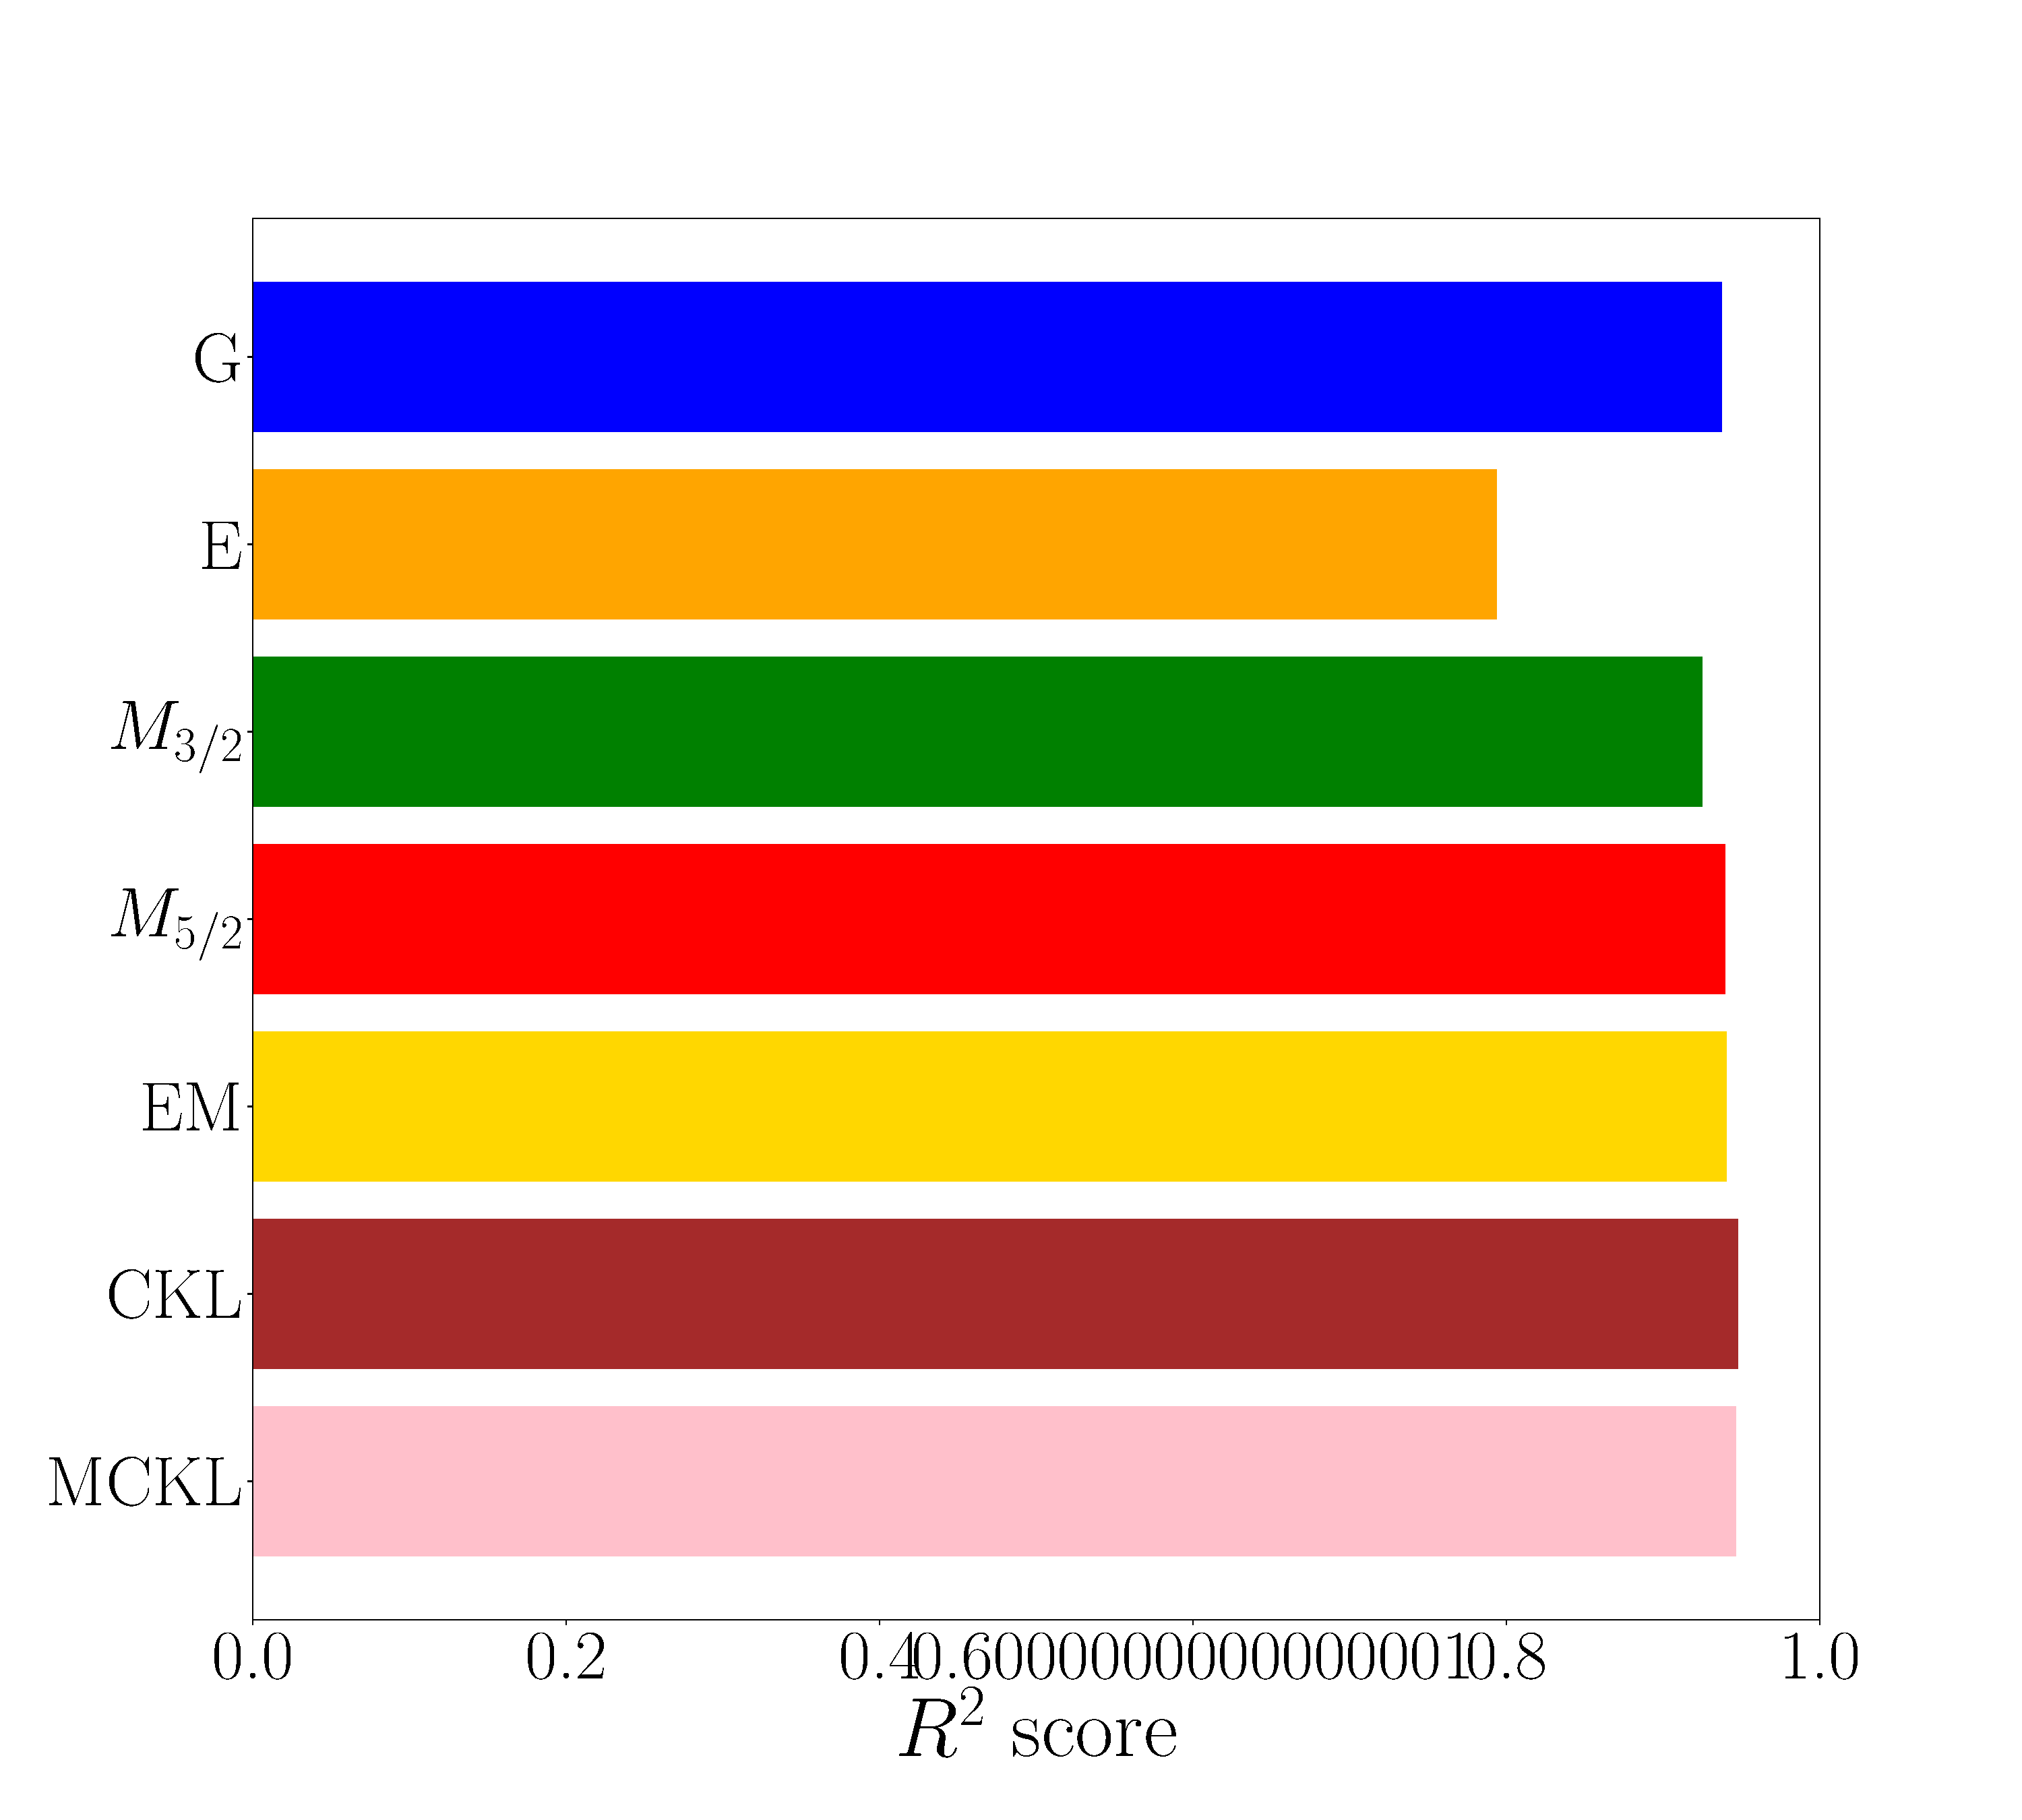
\includegraphics[width=0.50\textwidth,
				trim=0.25cm 0.25cm 0.25cm 0.25cm,
				clip]{figures/single_8D_R2.pdf}} 
			\subfloat[16D]{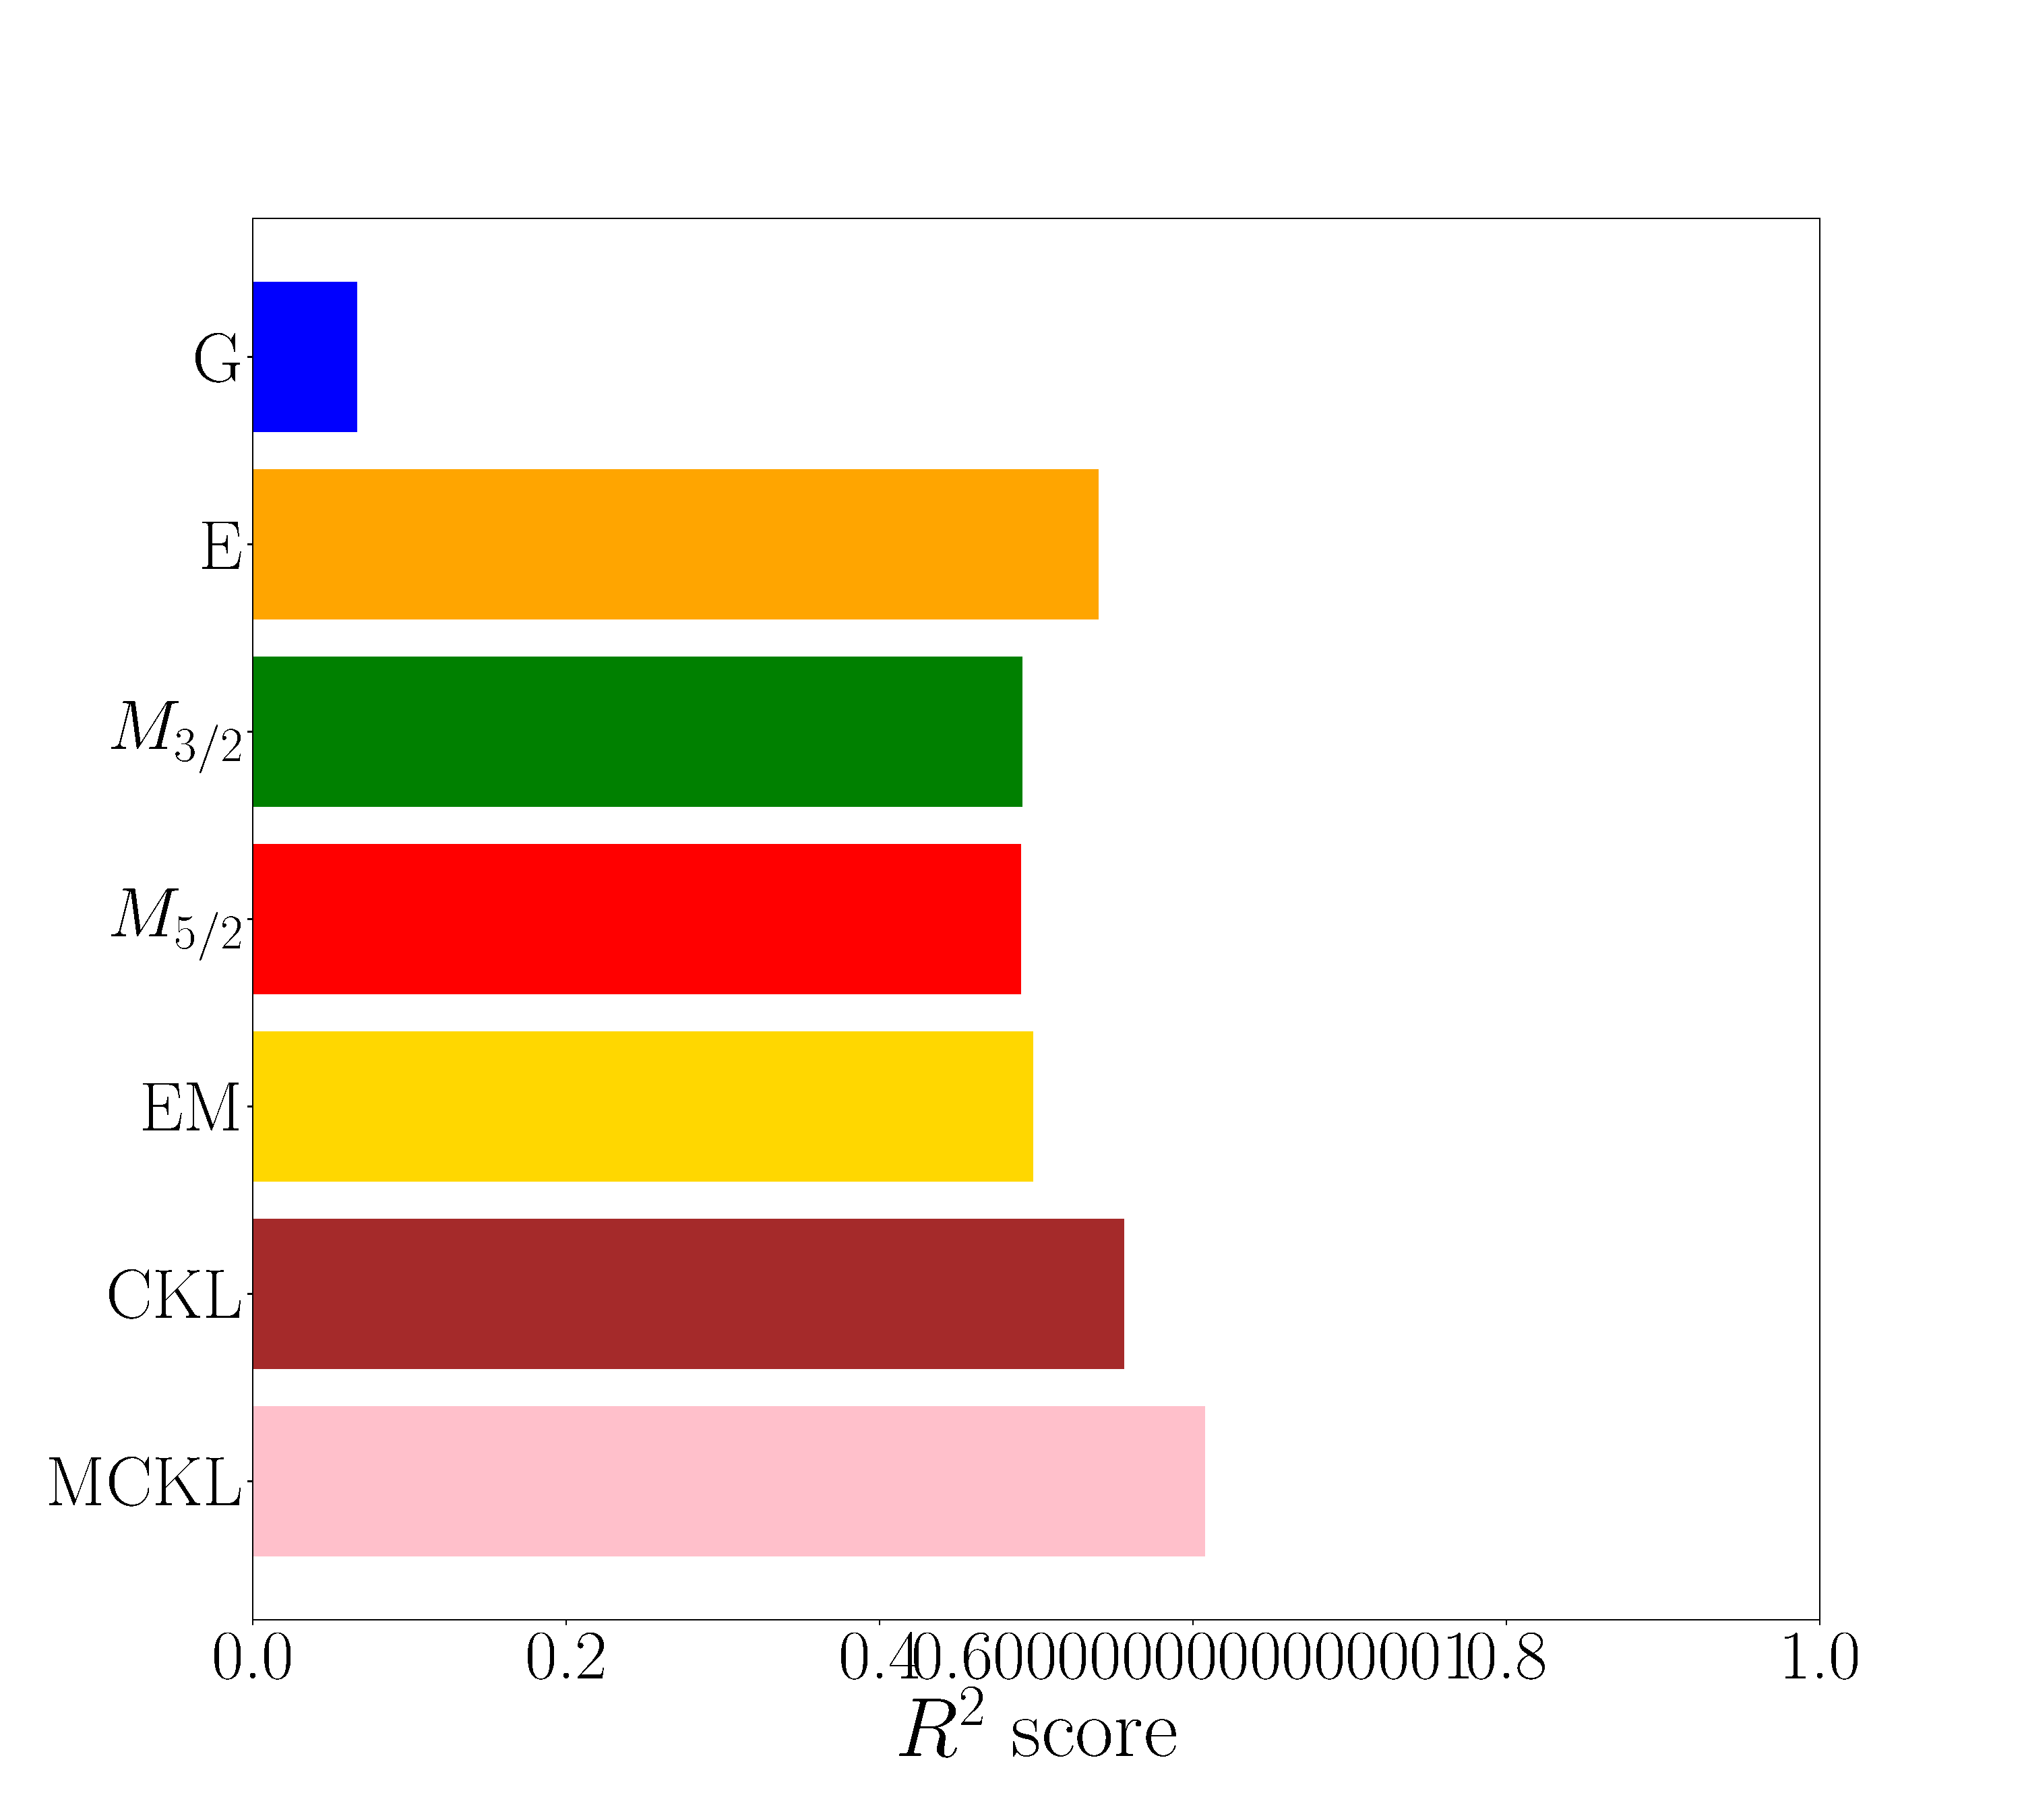
\includegraphics[width=0.50\textwidth,
				trim=0.25cm 0.25cm 0.25cm 0.25cm,
				clip]{figures/single_16D_R2.pdf}} }
		\caption{Coefficient of determination score of predictions}
		\label{fig:r2_score}
	\end{center}
\end{figure}

\begin{figure}[!h]
	\begin{center}
		\vspace{-10pt}
		\mbox{ \subfloat[8D]{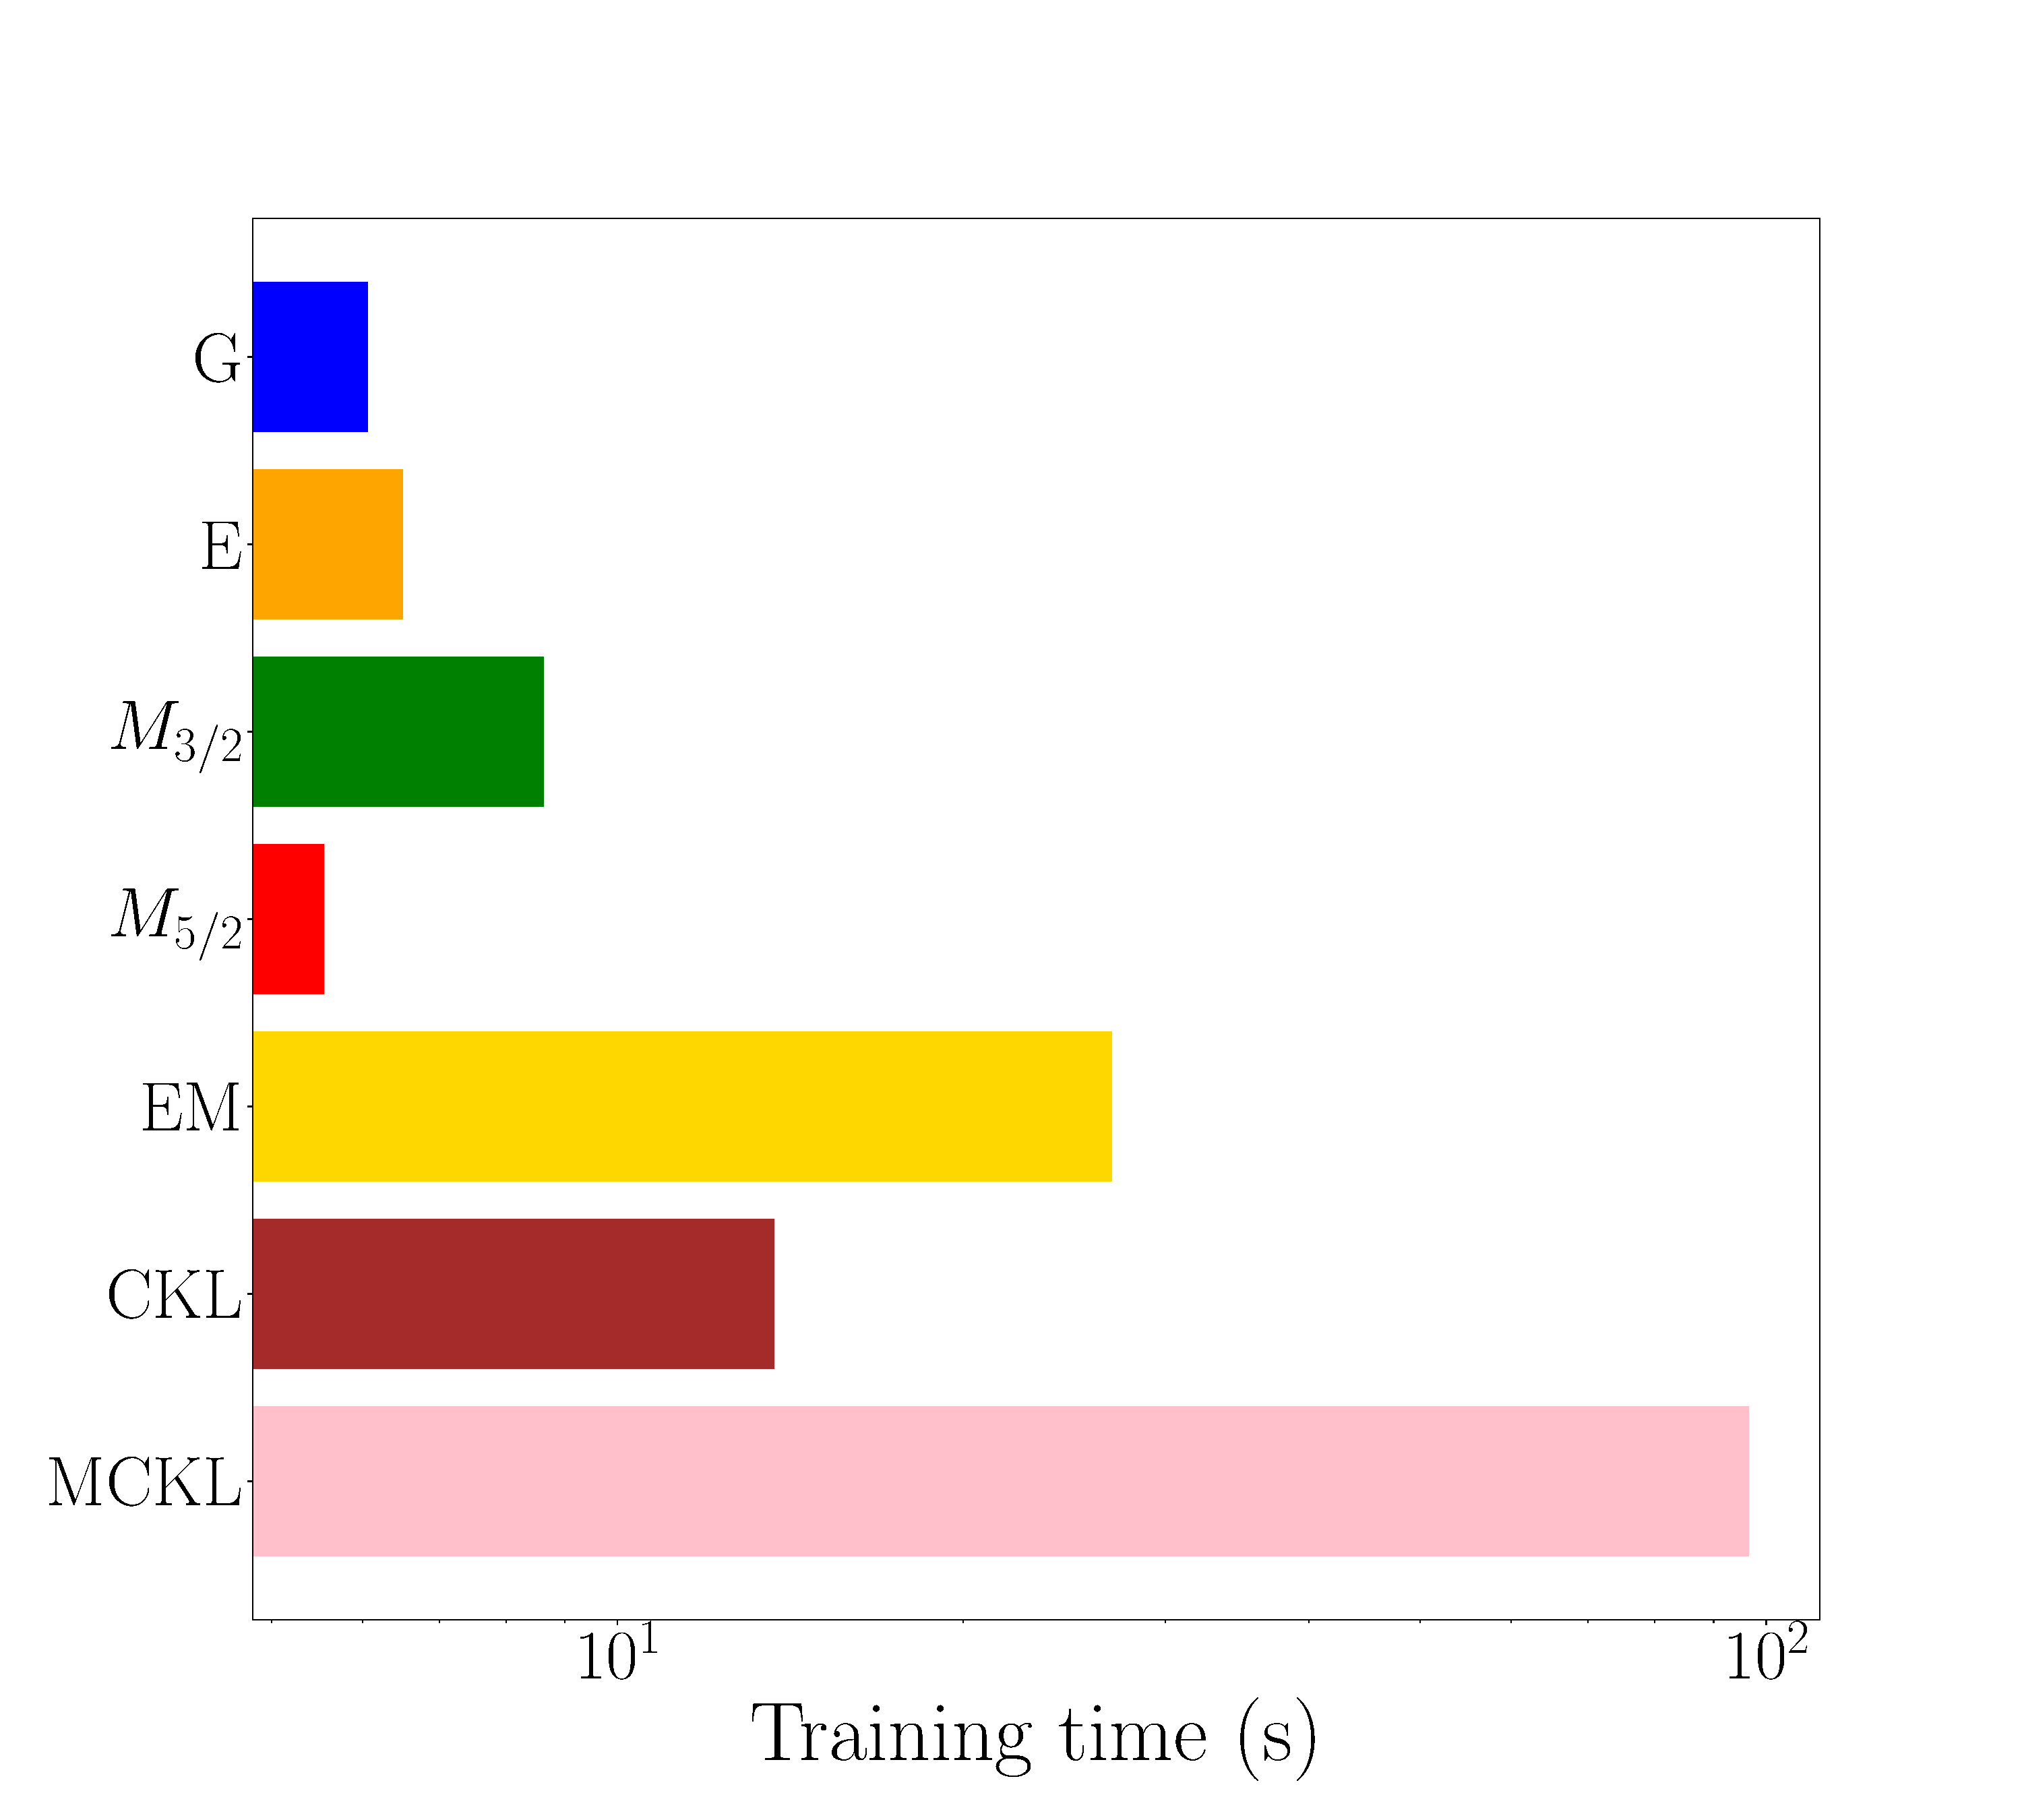
\includegraphics[width=0.50\textwidth,
				trim=0.25cm 0.25cm 0.25cm 0.25cm,
				clip]{figures/single_8D_training_time_n.pdf}} 
			\subfloat[16D]{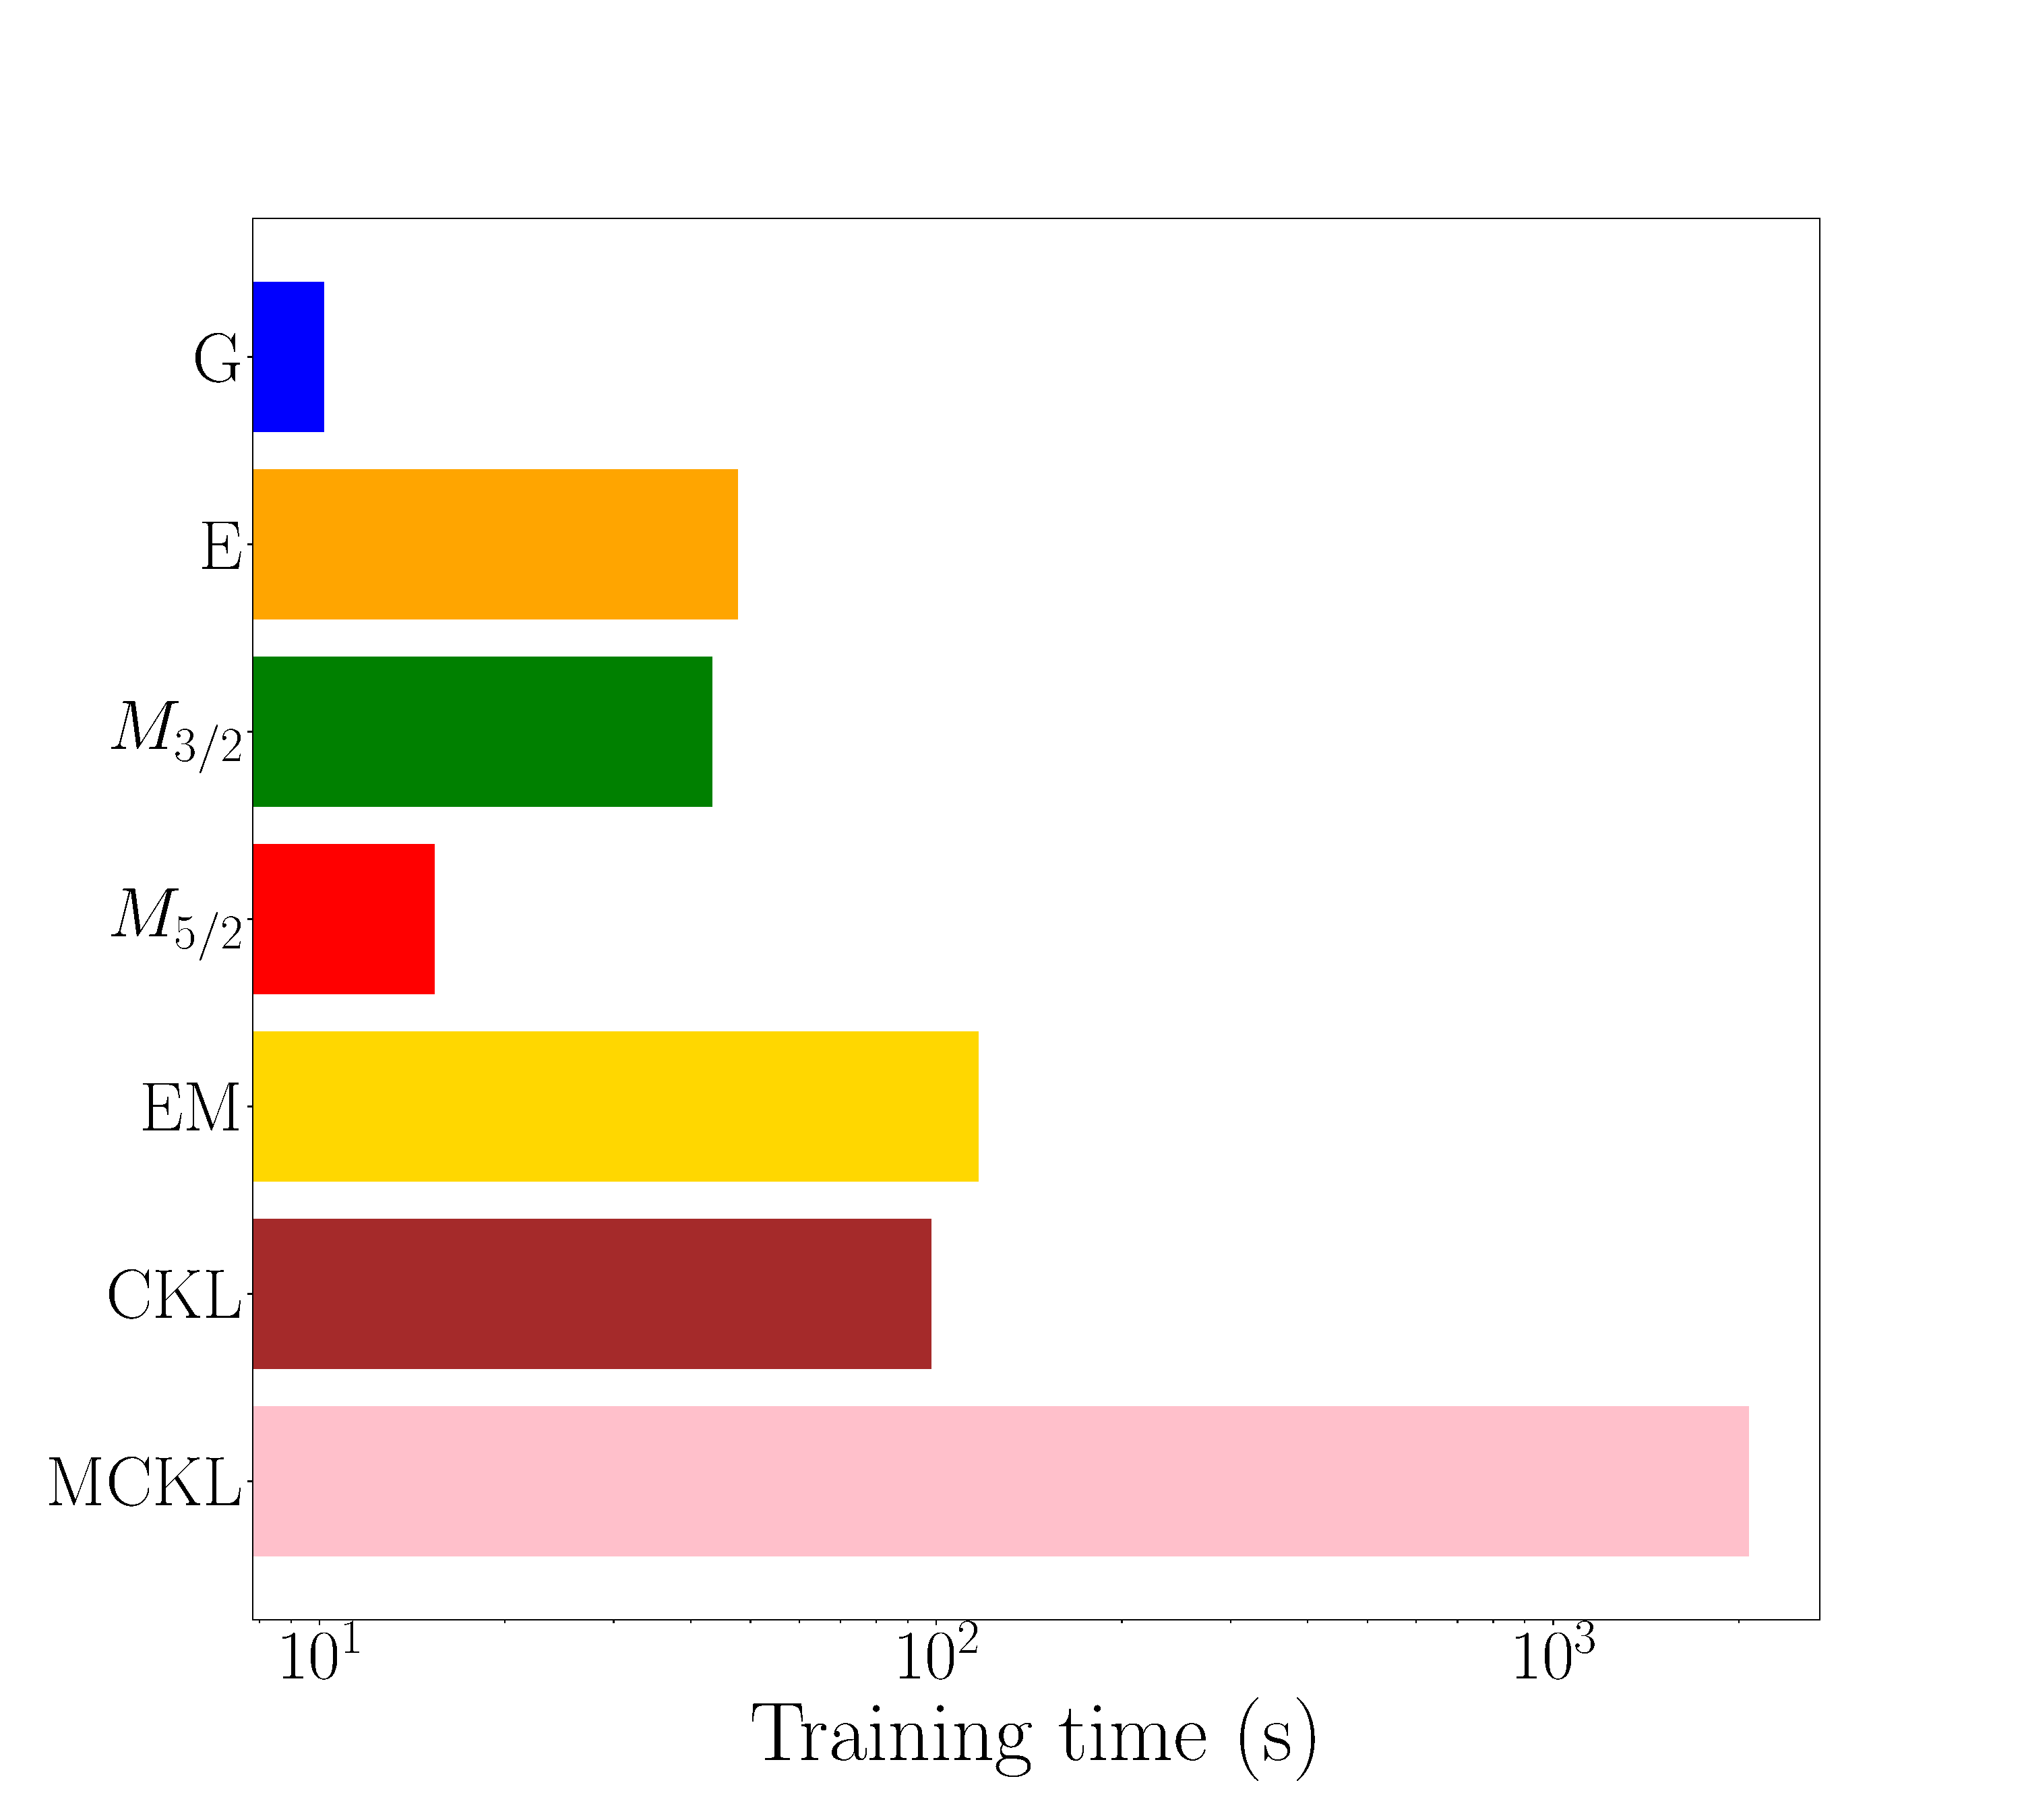
\includegraphics[width=0.50\textwidth,
				trim=0.25cm 0.25cm 0.25cm 0.25cm,
				clip]{figures/single_16D_training_time_n.pdf}} }
		\caption{Training time}
		\label{fig:training_time}
	\end{center}
\end{figure}

\section{Conclusion}
\subsection{Summary}
    \begin{itemize}
    \item Multiple kernel methods are more robust with better performance
    \item MCKL incurred the highest computational cost due to complexity of model
        \item CKL method is considered best for building models to predict drag coefficients
        \begin{itemize}
            \item Least training time for multiple kernel methods
            \item Reasonable model accuracy
        \end{itemize}
    \item The normalized root mean square method is a more reliable and interpretable metric for model performance comparison.
    \end{itemize}
    
\subsection{Contributions}
    \begin{enumerate}
        \item We developed a Halton-based sampling technique.
        \item We developed three multiple kernel learning methods based on weighting.
        \item We benchmarked performance of methods with single-kernel models.
    \end{enumerate}

\section{Reproducibility}
All the necessary files used to generate this report are available at \nolinkurl{https://github.com/kennybix/MATH_5470}.

% \clearpage
\begin{small}
\bibliography{references}{}
\bibliographystyle{plain}
\end{small}
\clearpage
 
\end{document}
